\documentclass[../main.tex]{subfiles}

\begin{document}

%%%%%%%%%%%%%%%%%%%%%%%%%%%%%%%%%%%
%
%	Average Read Depth Analysis Results
%
%%%%%%%%%%%%%%%%%%%%%%%%%%%%%%%%%%%

For all 15 strains of the \textit{Armillaria gallica} fungus the global average read depths and the total number of sites, based on the reference genome, are shown in table \ref{tab:avg_rd}.  

\begin{table}[H]
	\begin{center}
		\captionof{table}{Gobal Average Read Depths and Number of Reads for Each Strain} \label{tab:avg_rd}
		\vspace{0.5cm}
		\begin{tabular}{ |c|c|c| }
			\hline
			Strain & Global Average Read Depth & Total Global Number of Reads \\
			\hline
			Ar73 & 111.0507 & 69955093\\
			\hline
			Ar109 & 117.6863 & 70143802\\
			\hline
			Ar119 & 112.4868 & 70015910\\
			\hline
			Ar142 & 109.3741 & 70068064\\
			\hline
			Ar159 & 104.3773 & 69875550\\
			\hline
			Ar170 & 112.3987 & 70033946\\
			\hline
			Ar174 & 113.4283 & 70022954\\
			\hline
			Ar175 & 73.79959 & 69545937\\
			\hline
			Ar176 & 73.21531 & 69583274\\
			\hline
			Ar179 & 117.2196 & 70061598\\
			\hline
			Ar188 & 63.61699 & 68627951\\
			\hline
			Ar194 & 67.88522 & 69488072\\
			\hline
			Ar196 & 113.9182 & 70027951\\
			\hline
			Ar201 & 68.39596 & 69488227\\
			\hline
			Ar213 & 110.9612 & 69988055\\
			\hline
		\end{tabular}
	\end{center}
\end{table}

Table \ref{tab:avg_rd} shows that all fifteen strains which we can work with have a similar number of sites which reads were aligned to. This number of aligned reads was between 68.6 million and 70.1 million for all strains. The global average read depths (average read depth of all sites where reads were aligned) varied much more. The low end for global average read depths was for the strain Ar188 which had an average of 63.6 reads, when reads were aligned, and the high end for average read depth was 117.7 for the strain Ar109. Hao had mentioned that Ar 188 was not used in his analyses because it was different in some way to the other strains. Ar188 is the strain with the lowest number of reads and lowest total number of reads aligned.

The average number of reads within strains was also calculated, these results can be found in figures \ref{avg_rd_graphs_1}, \ref{avg_rd_graphs_2}, \ref{avg_rd_graphs_3}, \ref{avg_rd_graphs_4}, and \ref{avg_rd_graphs_5}. 

\begin{figure}[H]
	\begin{centering}
		\vspace{-1.5cm}
		\resizebox{78mm}{78mm}{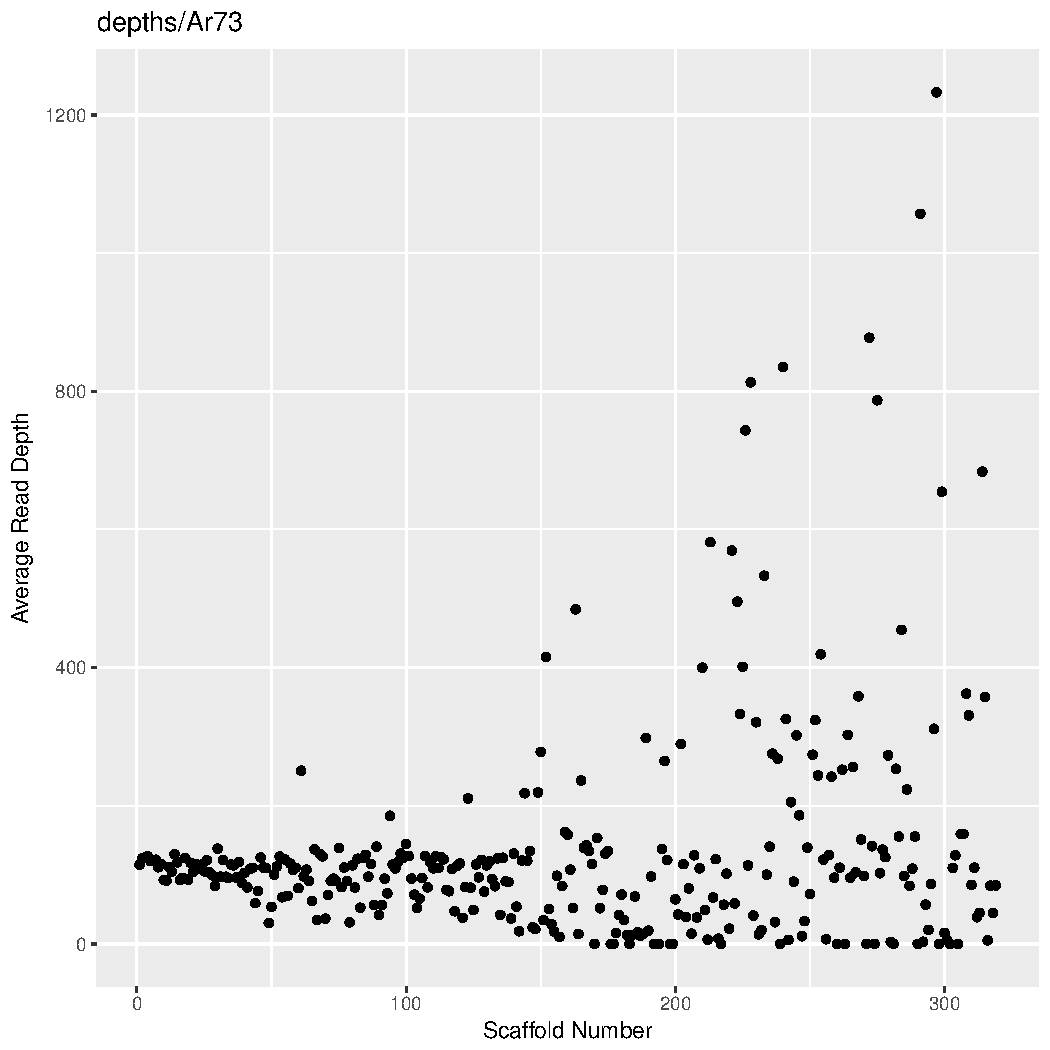
\includegraphics[angle=0,width=1.0\linewidth]{Figures/Ar73_collected_no_comma_read_depth.pdf}}
		\resizebox{78mm}{78mm}{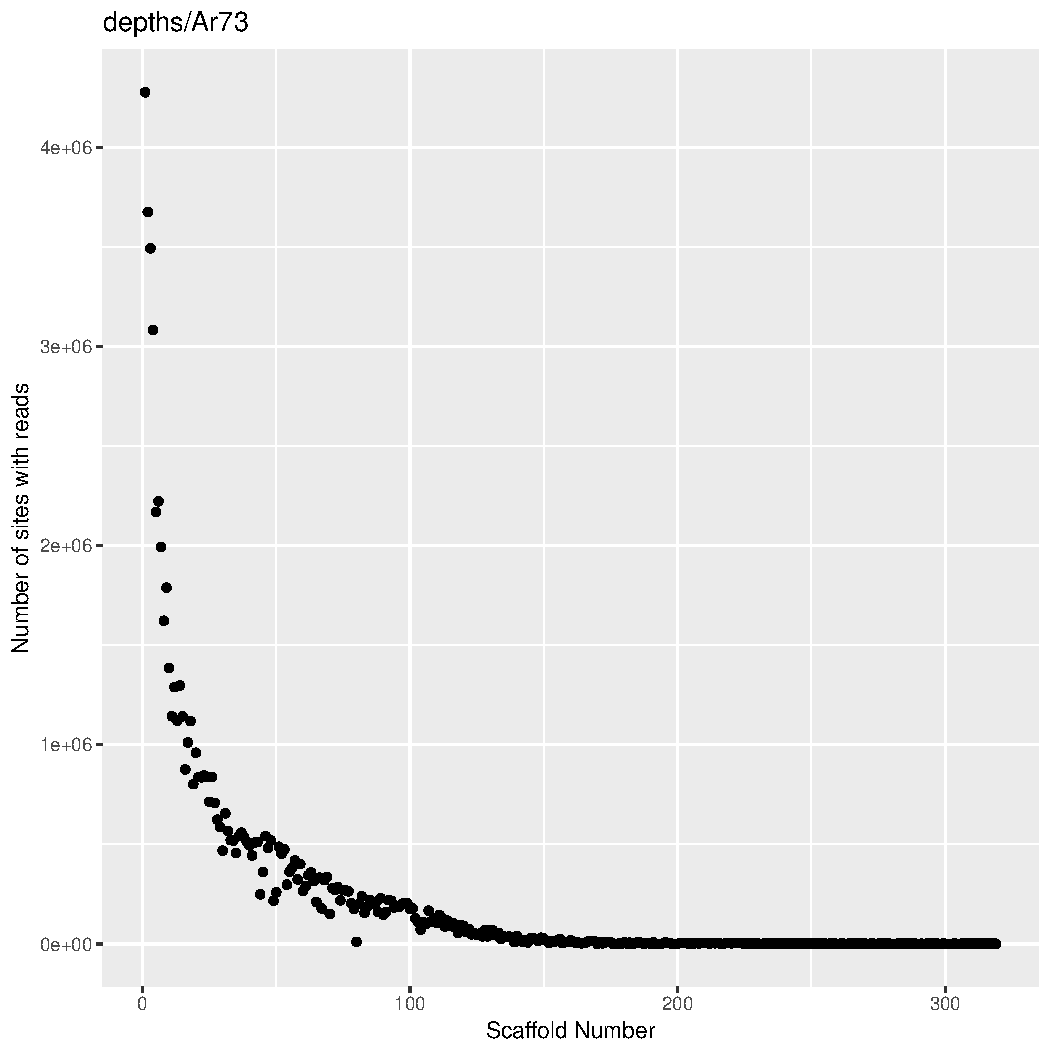
\includegraphics[angle=0,width=1.0\linewidth]{Figures/Ar73_collected_no_comma_count.pdf}}\\
		\resizebox{78mm}{78mm}{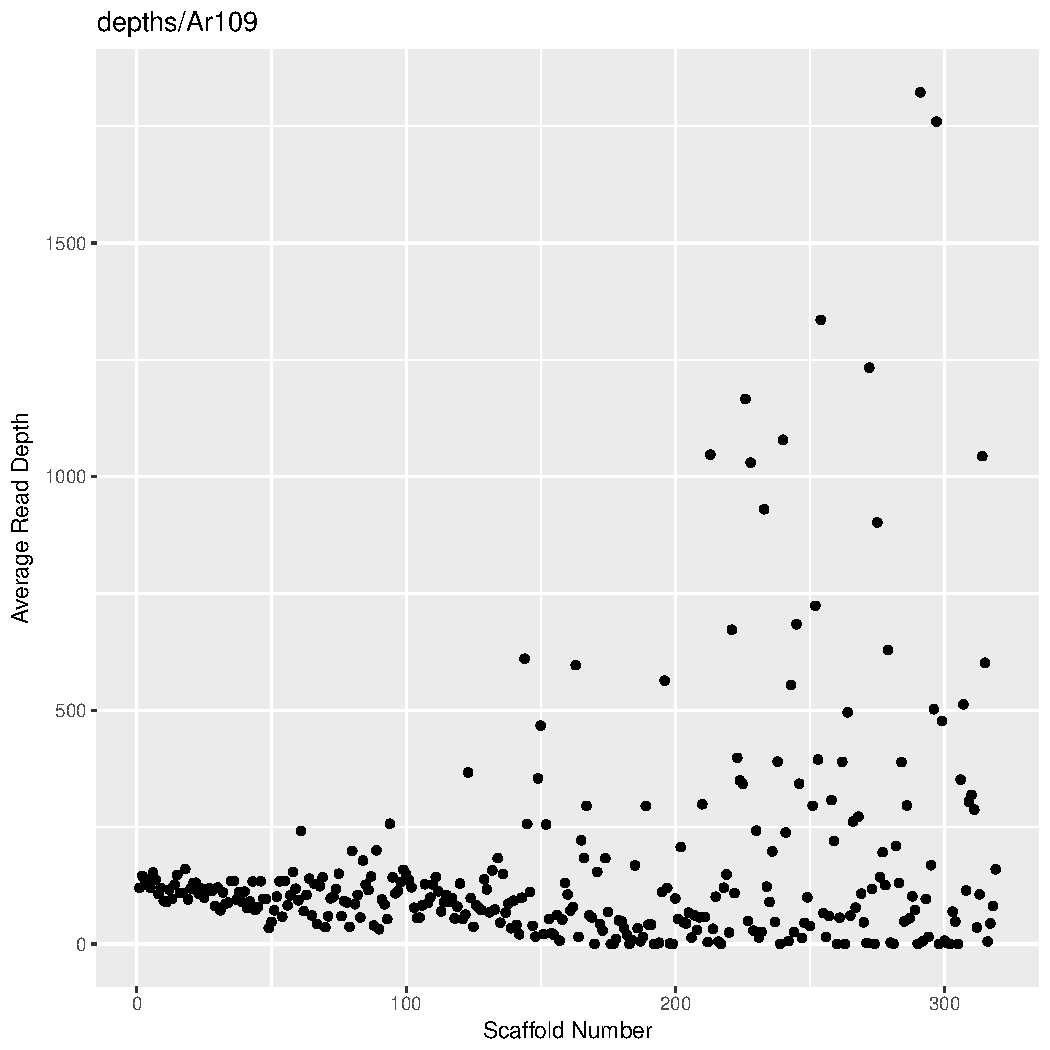
\includegraphics[angle=0,width=1.0\linewidth]{Figures/Ar109_collected_no_comma_read_depth.pdf}}
		\resizebox{78mm}{78mm}{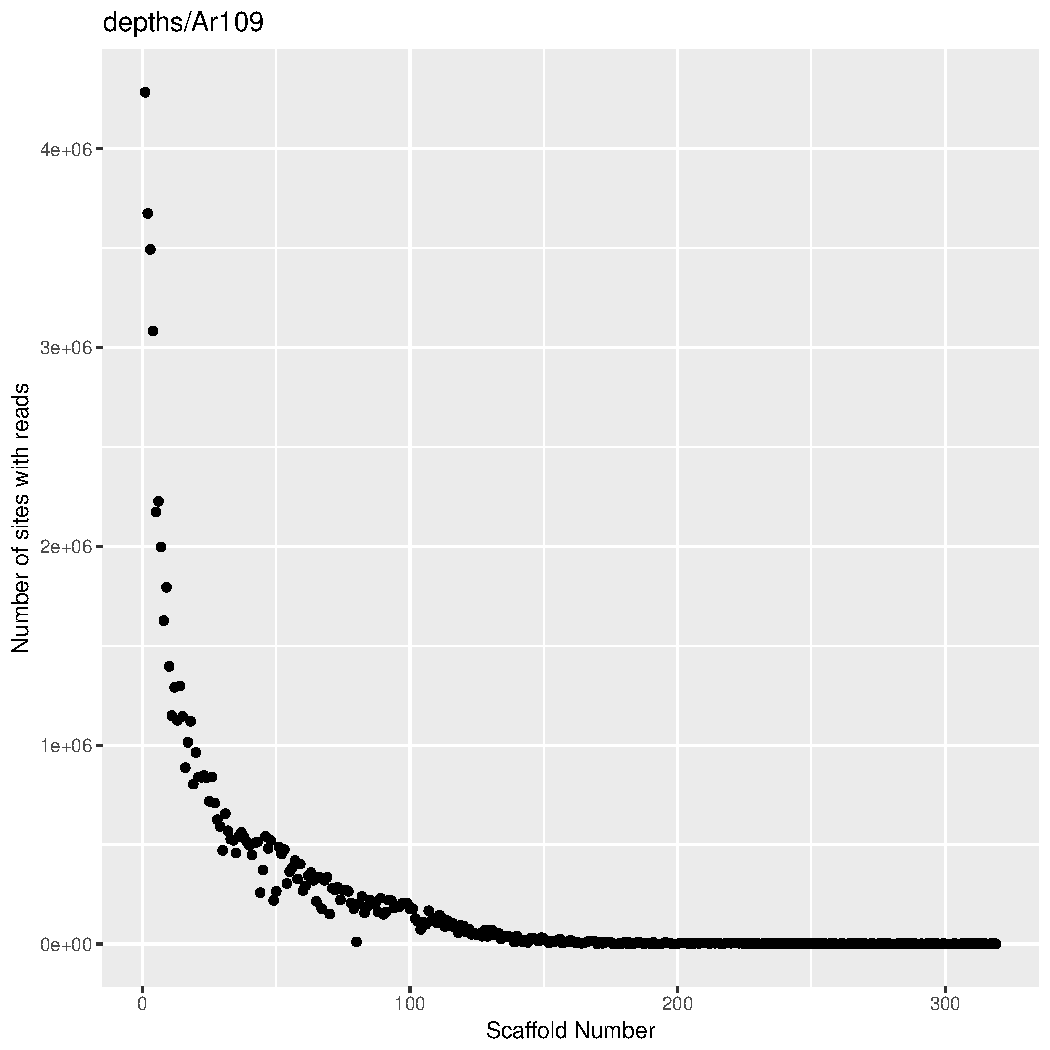
\includegraphics[angle=0,width=1.0\linewidth]{Figures/Ar109_collected_no_comma_count.pdf}}\\
		\resizebox{78mm}{78mm}{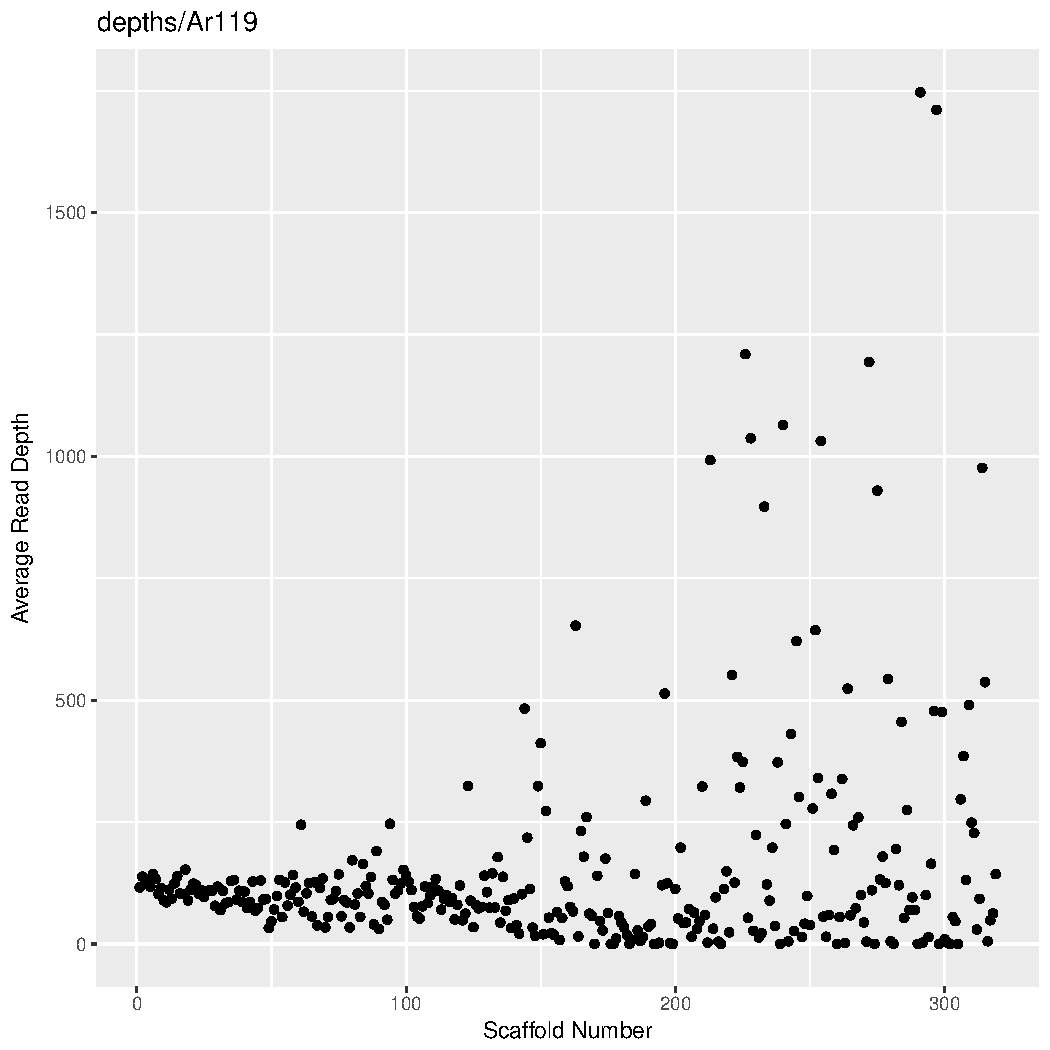
\includegraphics[angle=0,width=1.0\linewidth]{Figures/Ar119_collected_no_comma_read_depth.pdf}}
		\resizebox{78mm}{78mm}{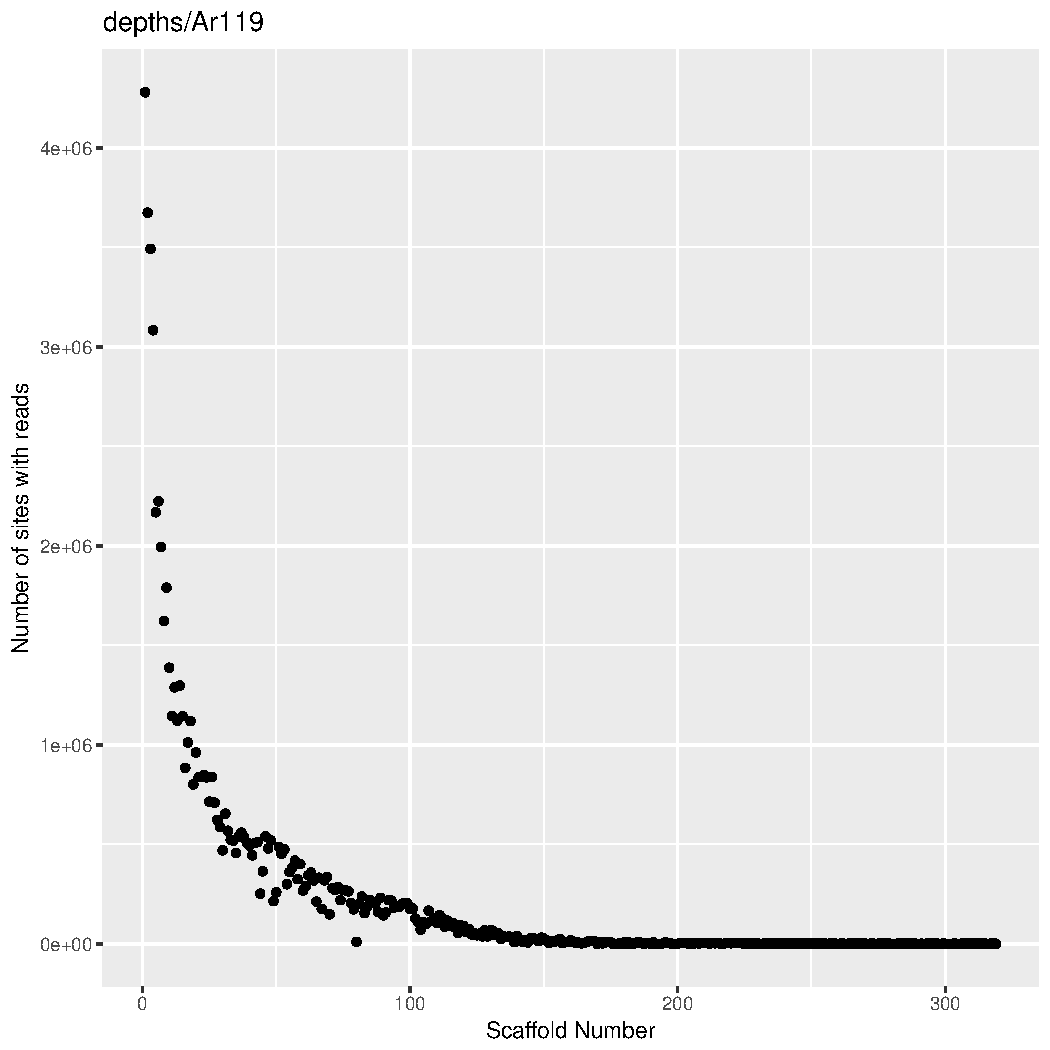
\includegraphics[angle=0,width=1.0\linewidth]{Figures/Ar119_collected_no_comma_count.pdf}}\\
		\begin{singlespace}
			\vspace{-0.5cm}
			\caption[Average Read Depth Per scaffold, Ar:73, 109, 119]{Average Read Depth Per scaffold, Ar:73, 109, 119. Graphs on the left are the average read depth vs scaffold number and graphs on the right are the total number of sites with reads aligned to them per scaffold.}\label{avg_rd_graphs_1}
		\end{singlespace}
	\end{centering}
\end{figure}
\begin{figure}[H]
	\begin{centering}
		\vspace{-1.5cm}
		\resizebox{78mm}{78mm}{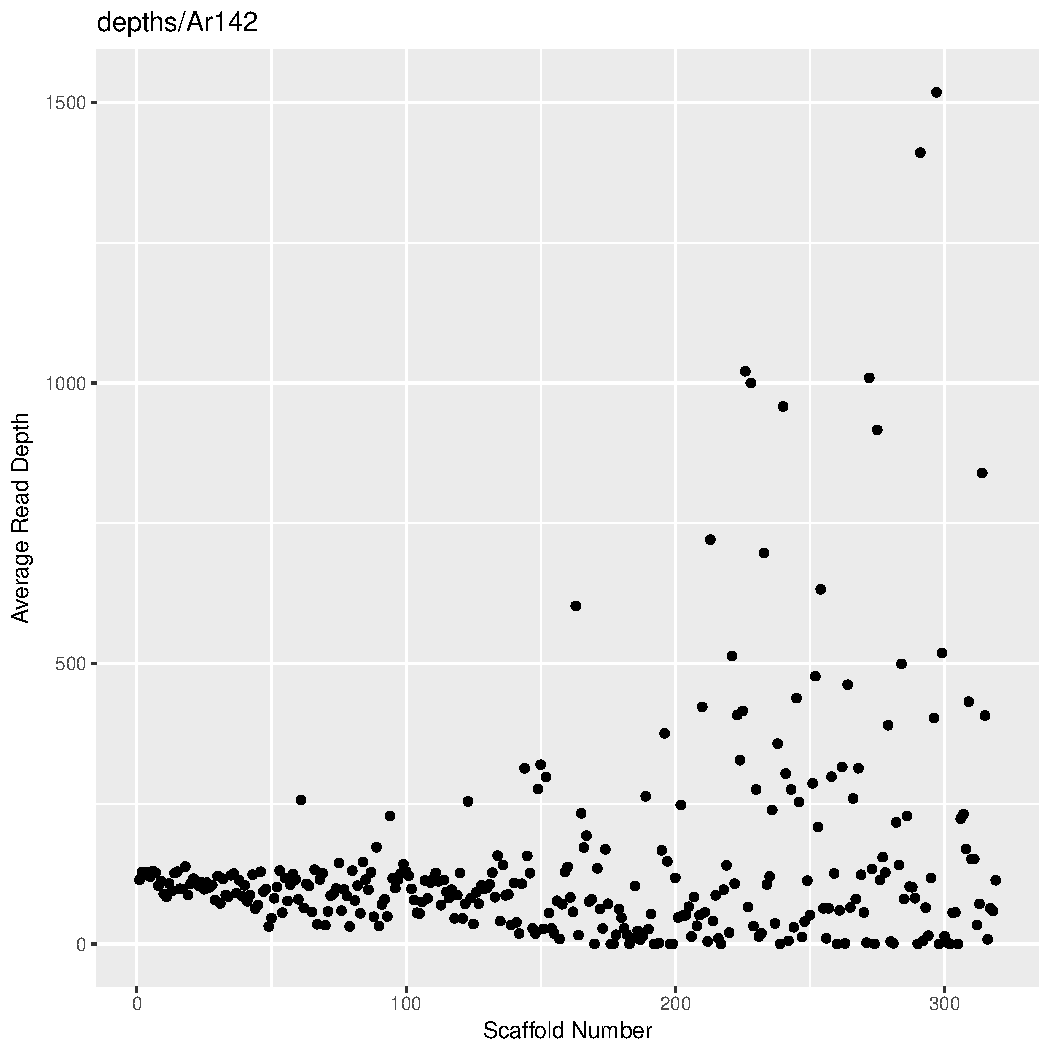
\includegraphics[angle=0,width=1.0\linewidth]{Figures/Ar142_collected_no_comma_read_depth.pdf}}
		\resizebox{78mm}{78mm}{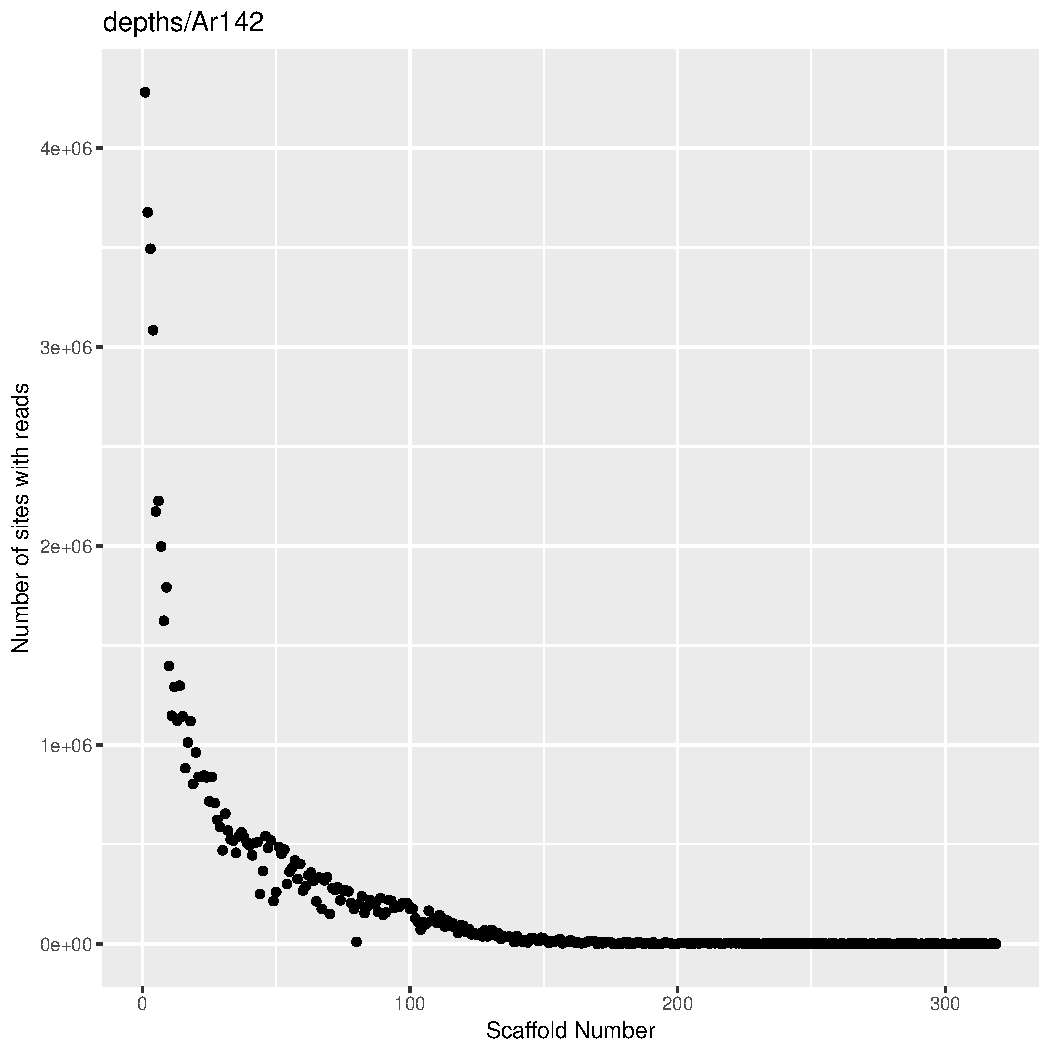
\includegraphics[angle=0,width=1.0\linewidth]{Figures/Ar142_collected_no_comma_count.pdf}}\\
		\resizebox{78mm}{78mm}{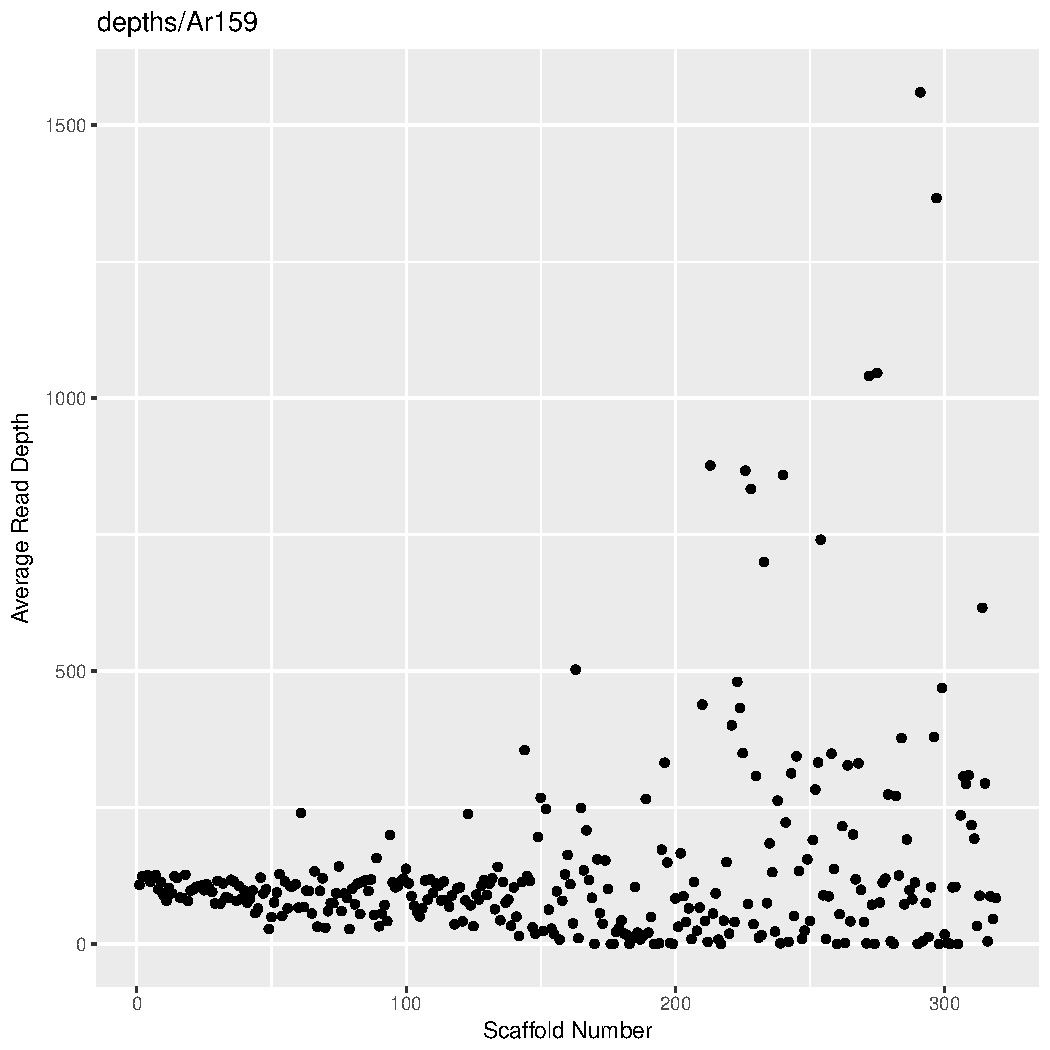
\includegraphics[angle=0,width=1.0\linewidth]{Figures/Ar159_collected_no_comma_read_depth.pdf}}
		\resizebox{78mm}{78mm}{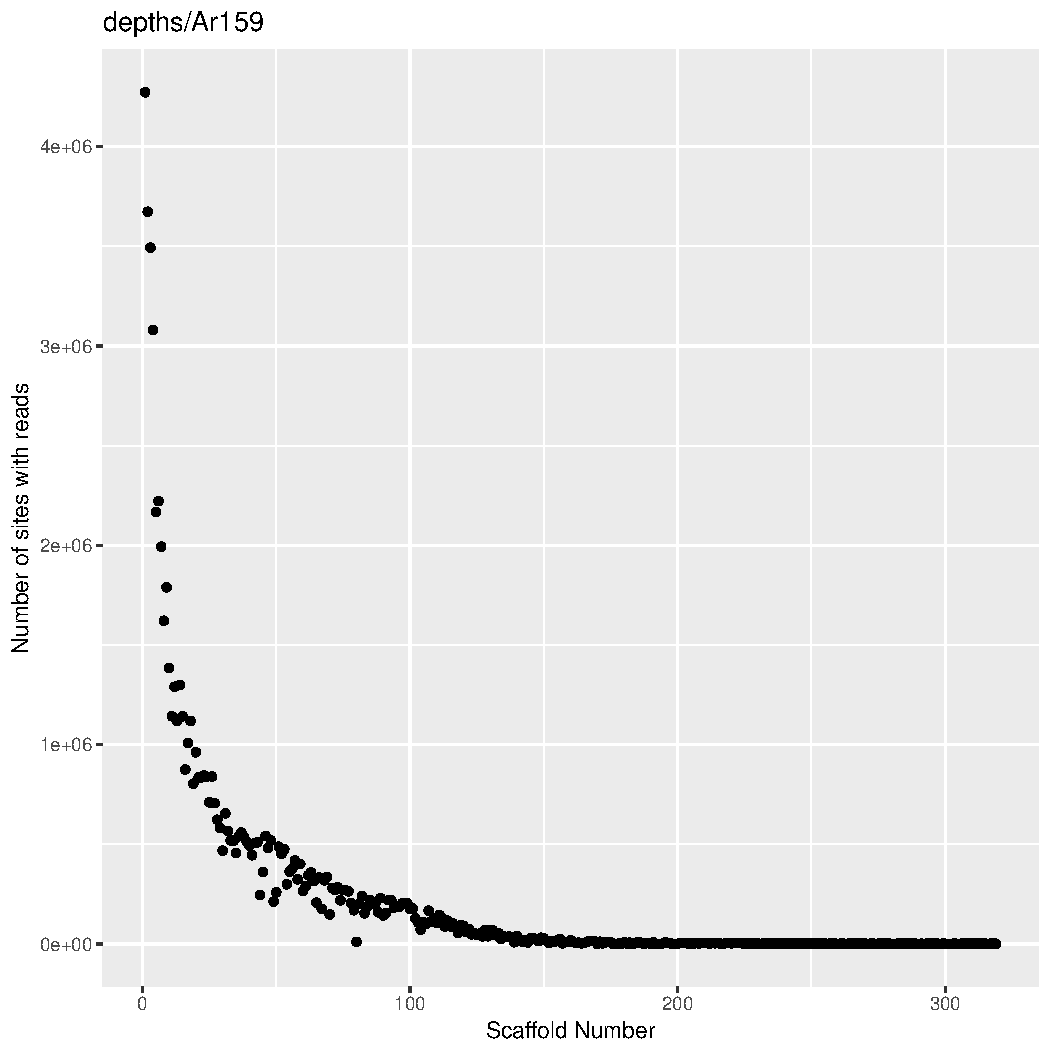
\includegraphics[angle=0,width=1.0\linewidth]{Figures/Ar159_collected_no_comma_count.pdf}}\\
		\resizebox{78mm}{78mm}{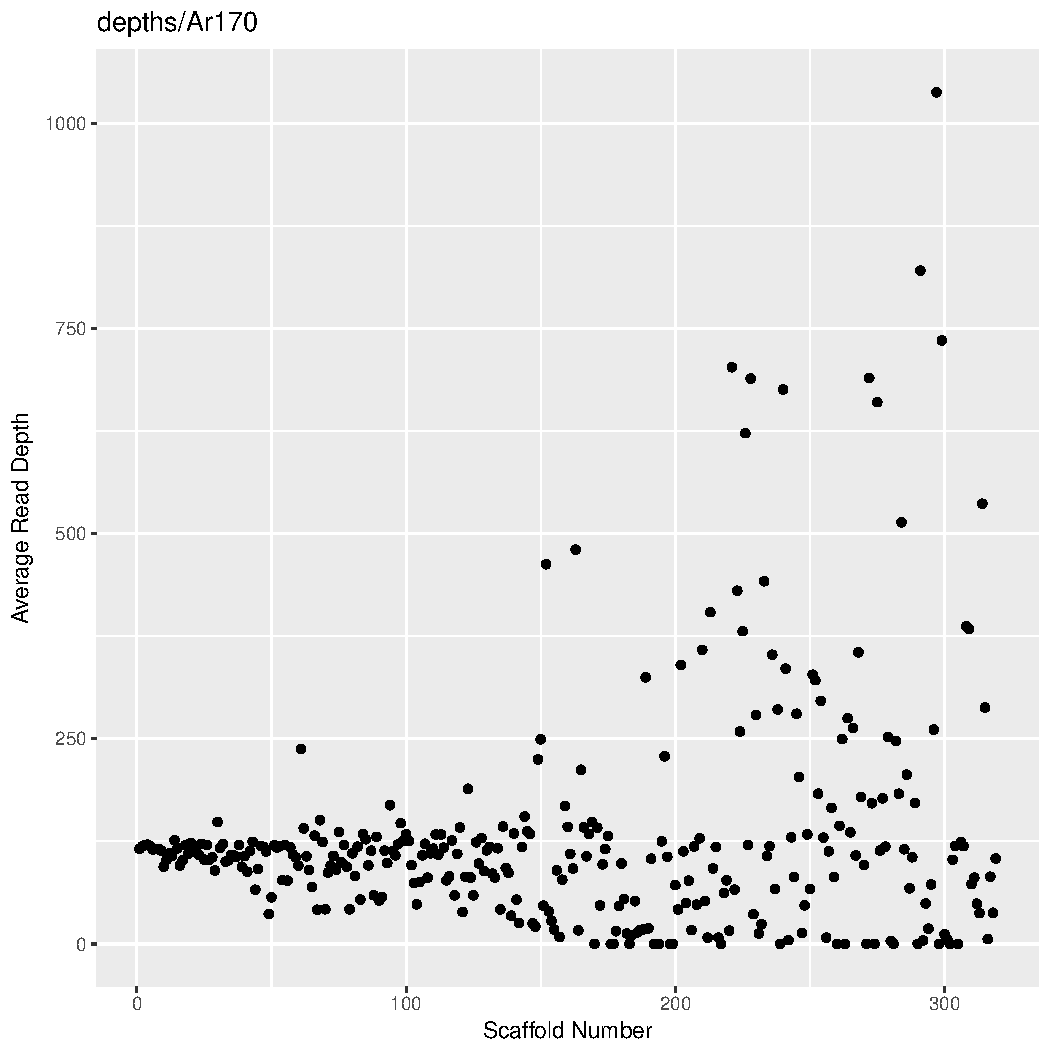
\includegraphics[angle=0,width=1.0\linewidth]{Figures/Ar170_collected_no_comma_read_depth.pdf}}
		\resizebox{78mm}{78mm}{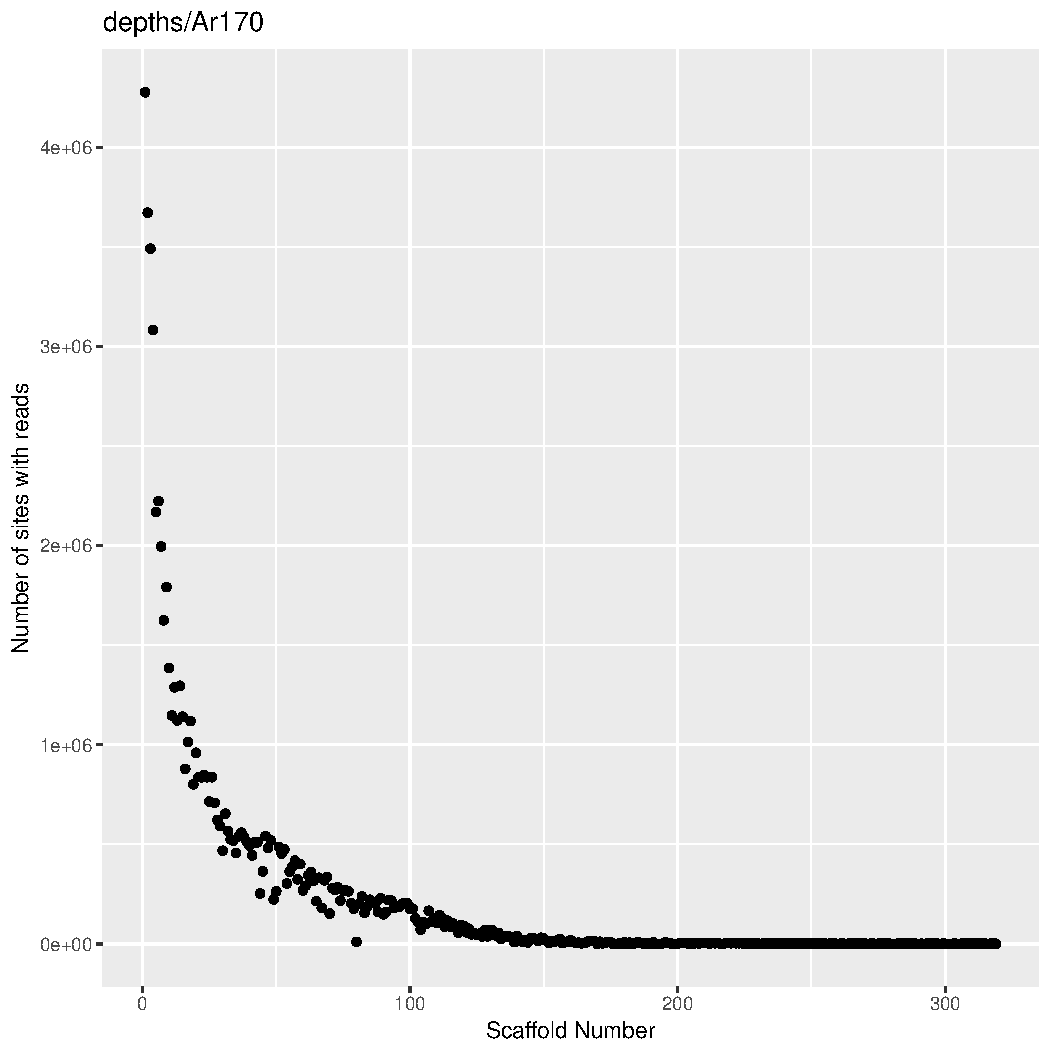
\includegraphics[angle=0,width=1.0\linewidth]{Figures/Ar170_collected_no_comma_count.pdf}}\\
		\begin{singlespace}
			\vspace{-0.5cm}
			\caption[Average Read Depth Per scaffold, Ar: 142, 159, 170]{Average Read Depth Per scaffold, Ar: 142, 159, 170. Graphs on the left are the average read depth vs scaffold number and graphs on the right are the total number of sites with reads aligned to them per scaffold.}\label{avg_rd_graphs_2}
		\end{singlespace}
	\end{centering}
\end{figure}
\begin{figure}[H]
	\begin{centering}
		\vspace{-1.5cm}
		\resizebox{78mm}{78mm}{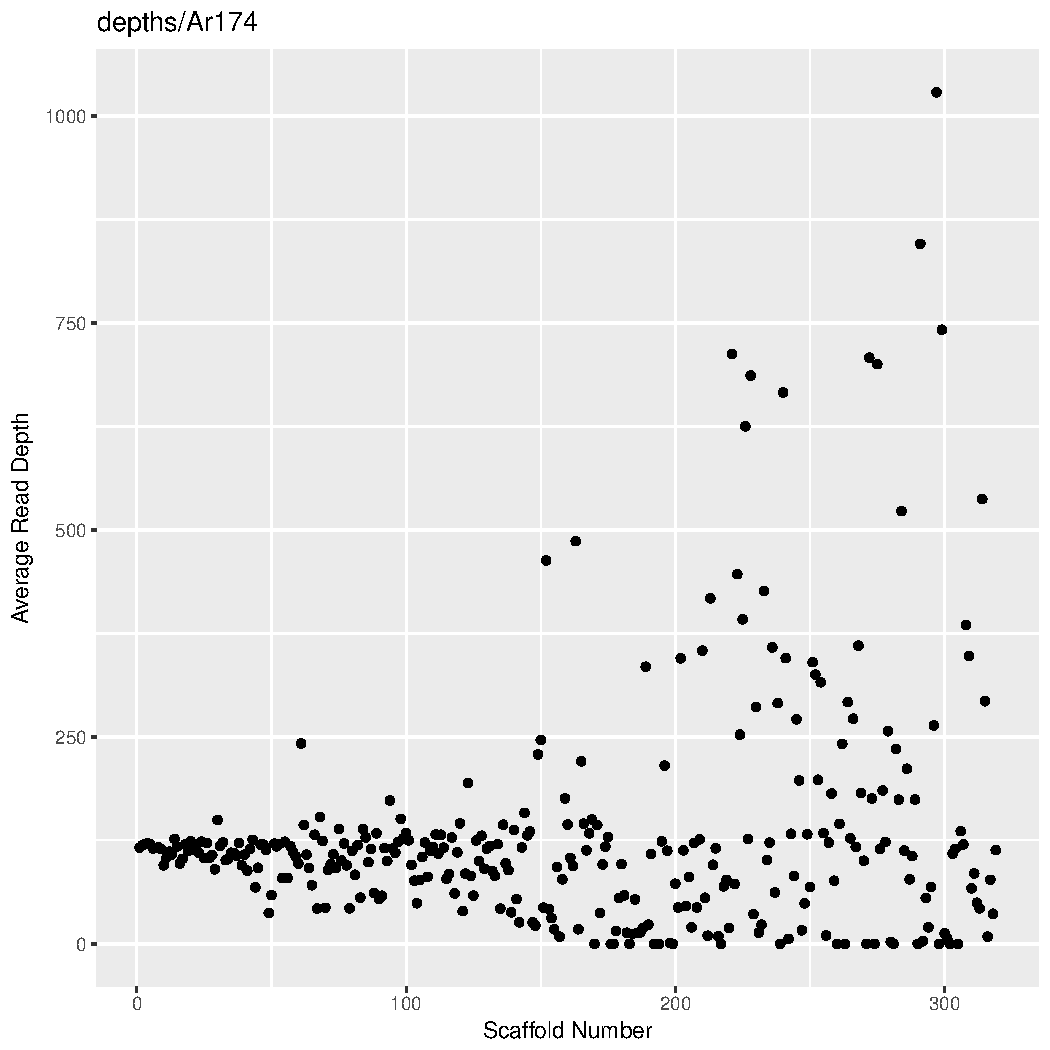
\includegraphics[angle=0,width=1.0\linewidth]{Figures/Ar174_collected_no_comma_read_depth.pdf}}
		\resizebox{78mm}{78mm}{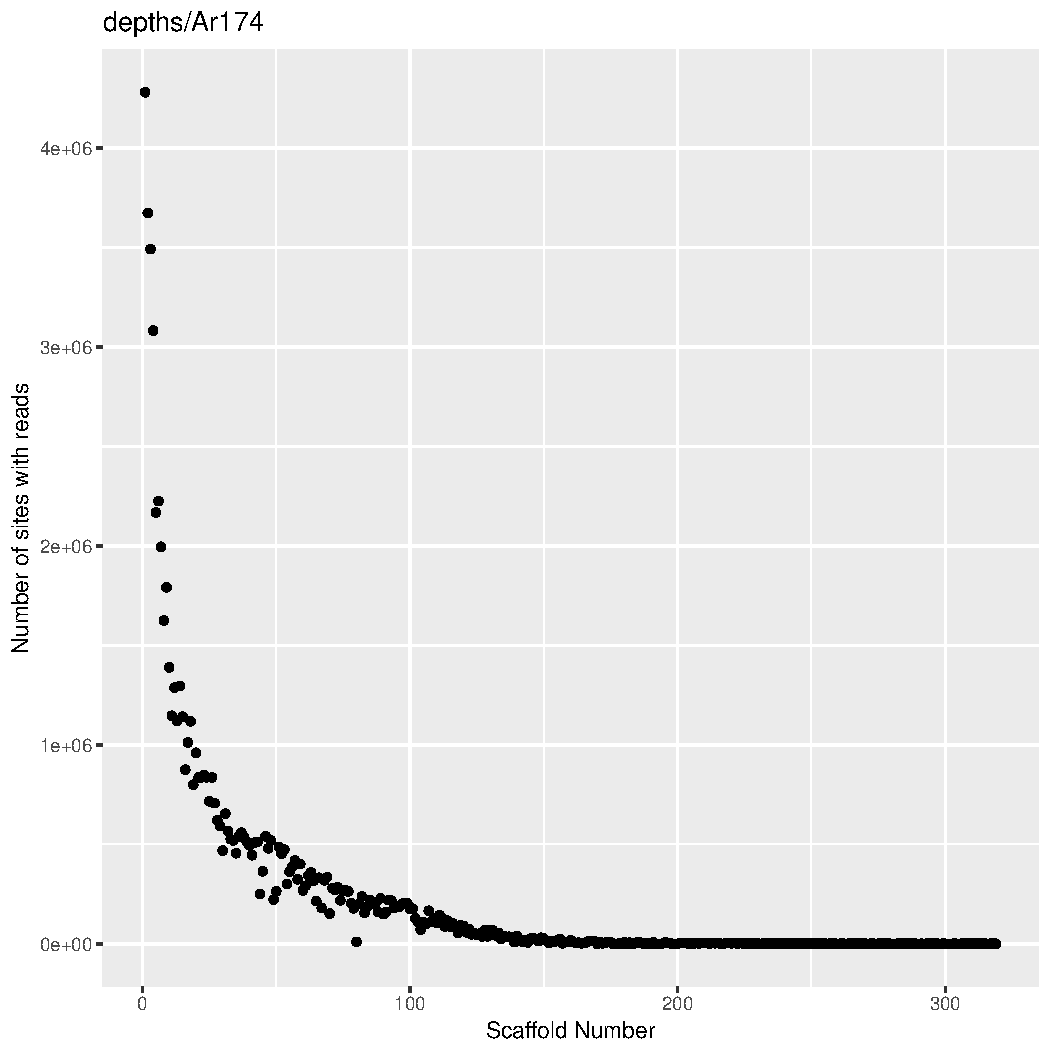
\includegraphics[angle=0,width=1.0\linewidth]{Figures/Ar174_collected_no_comma_count.pdf}}\\
		\resizebox{78mm}{78mm}{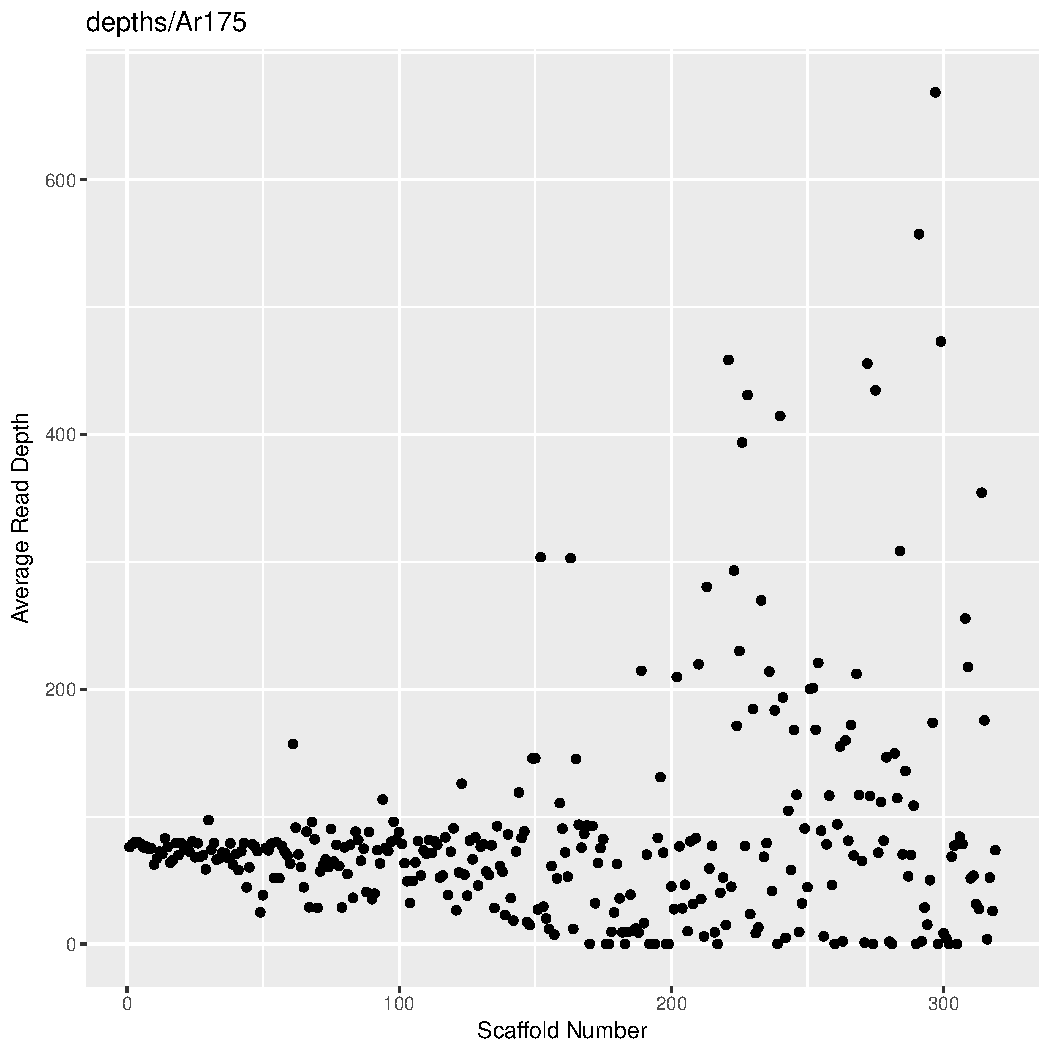
\includegraphics[angle=0,width=1.0\linewidth]{Figures/Ar175_collected_no_comma_read_depth.pdf}}
		\resizebox{78mm}{78mm}{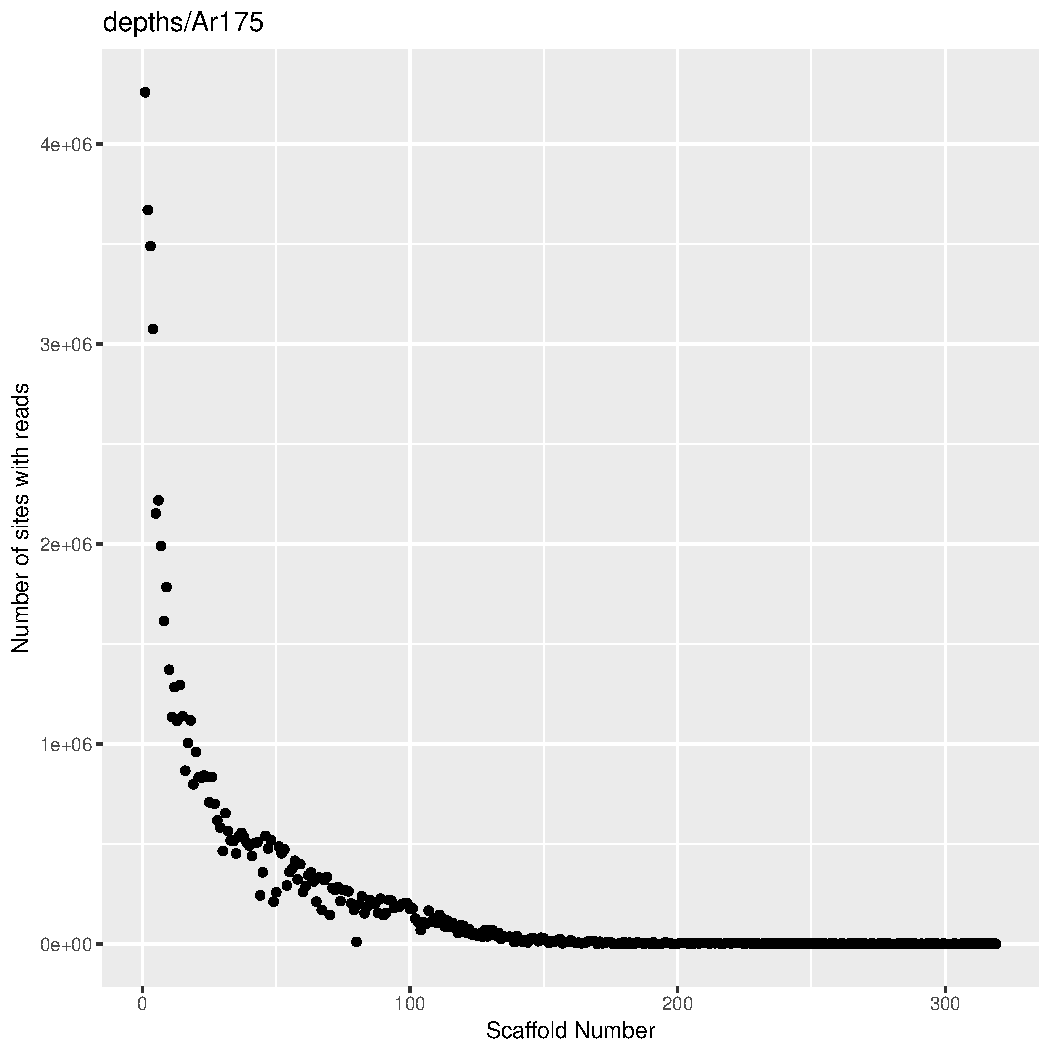
\includegraphics[angle=0,width=1.0\linewidth]{Figures/Ar175_collected_no_comma_count.pdf}}\\
		\resizebox{78mm}{78mm}{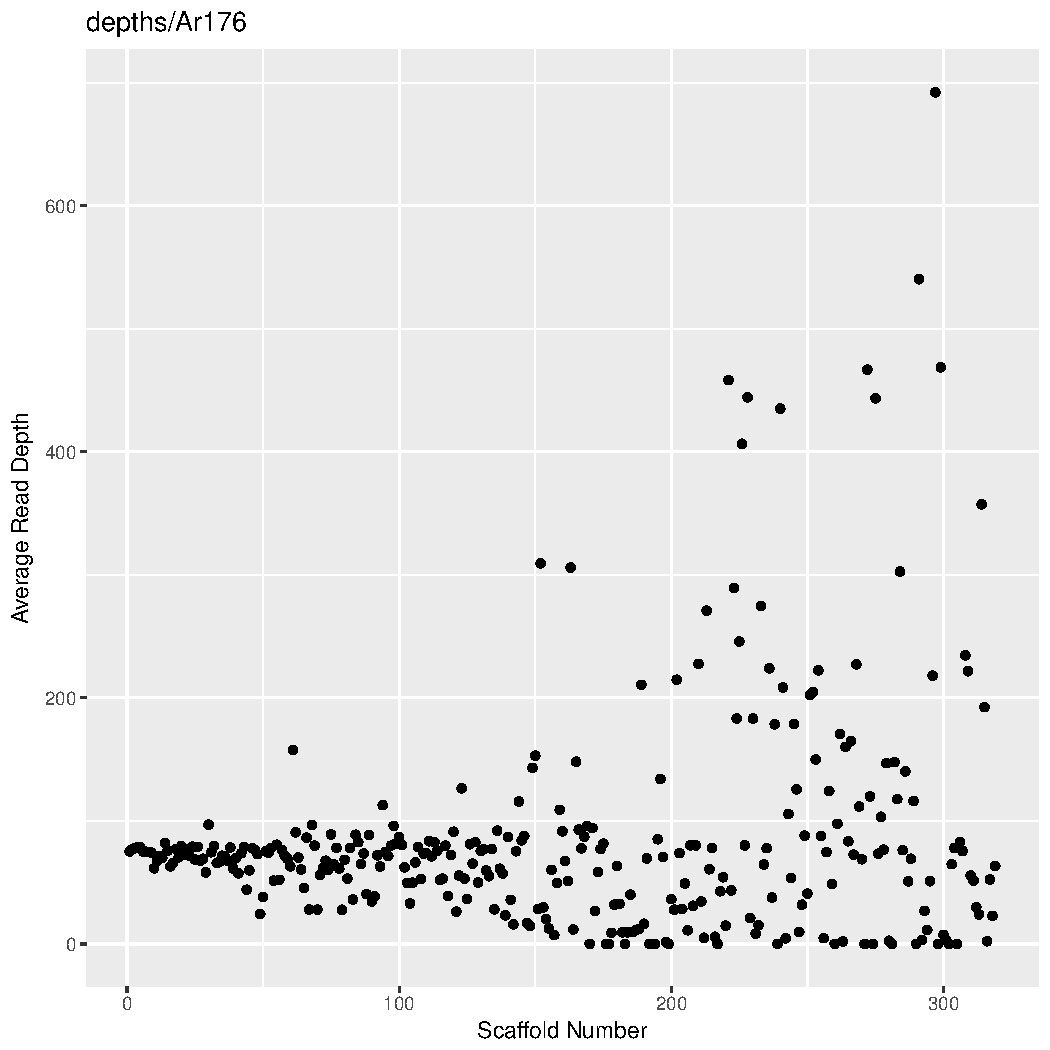
\includegraphics[angle=0,width=1.0\linewidth]{Figures/Ar176_collected_no_comma_read_depth.pdf}}
		\resizebox{78mm}{78mm}{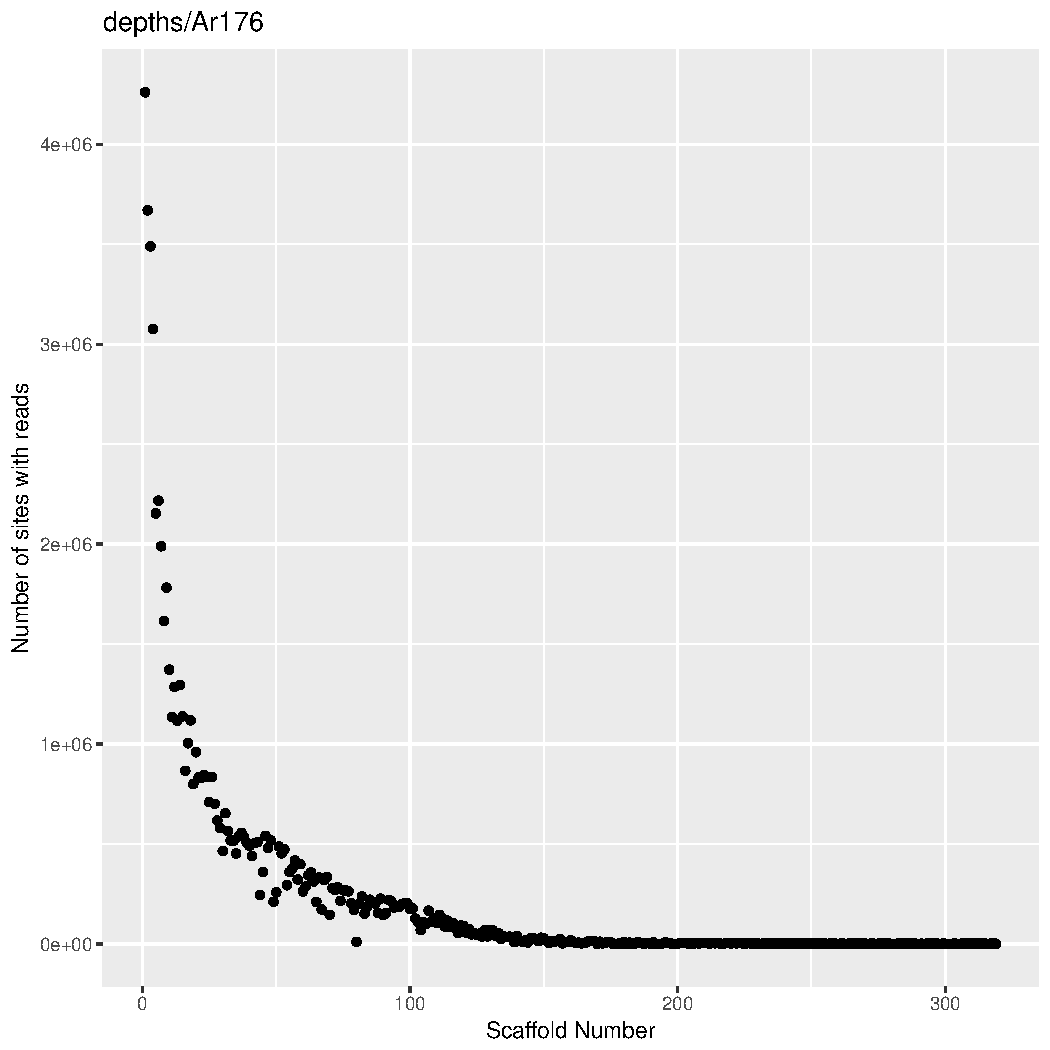
\includegraphics[angle=0,width=1.0\linewidth]{Figures/Ar176_collected_no_comma_count.pdf}}\\
		\begin{singlespace}
			\vspace{-0.5cm}
			\caption[Average Read Depth Per scaffold, Ar:174, 175, 176]{Average Read Depth Per scaffold, Ar:174, 175, 176. Graphs on the left are the average read depth vs scaffold number and graphs on the right are the total number of sites with reads aligned to them per scaffold.}\label{avg_rd_graphs_3}
		\end{singlespace}	
	\end{centering}
\end{figure}
\begin{figure}[H]
	\begin{centering}
		\vspace{-1.5cm}
		\resizebox{78mm}{78mm}{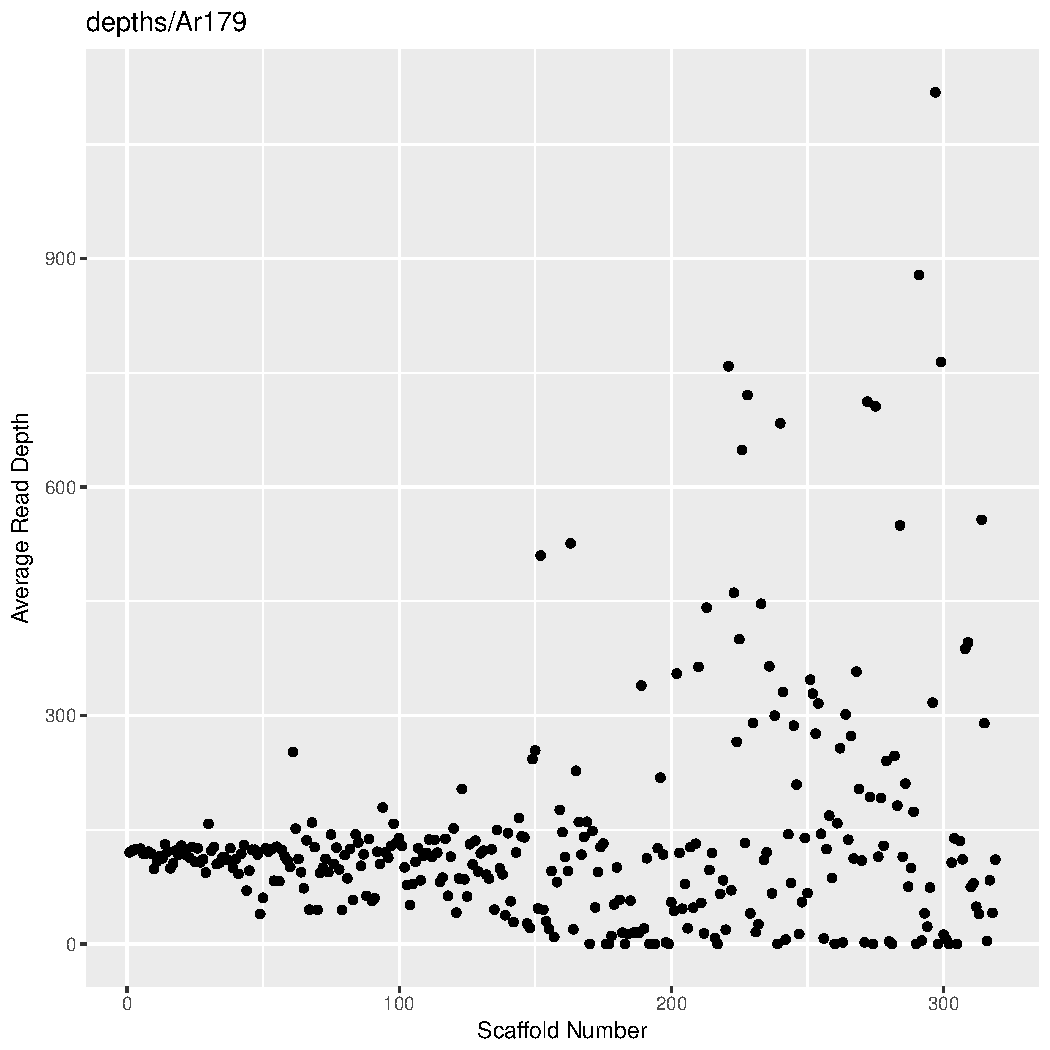
\includegraphics[angle=0,width=1.0\linewidth]{Figures/Ar179_collected_no_comma_read_depth.pdf}}
		\resizebox{78mm}{78mm}{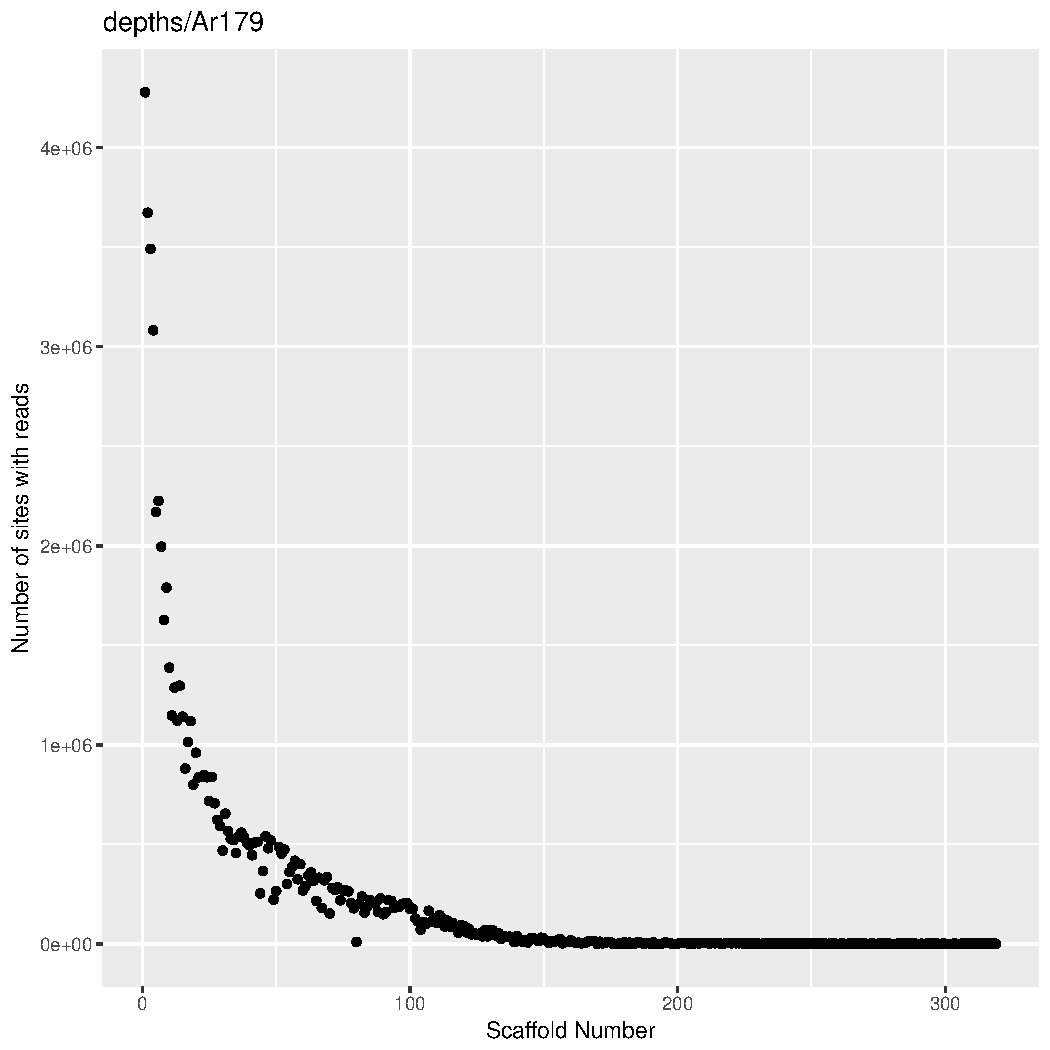
\includegraphics[angle=0,width=1.0\linewidth]{Figures/Ar179_collected_no_comma_count.pdf}}\\
		\resizebox{78mm}{78mm}{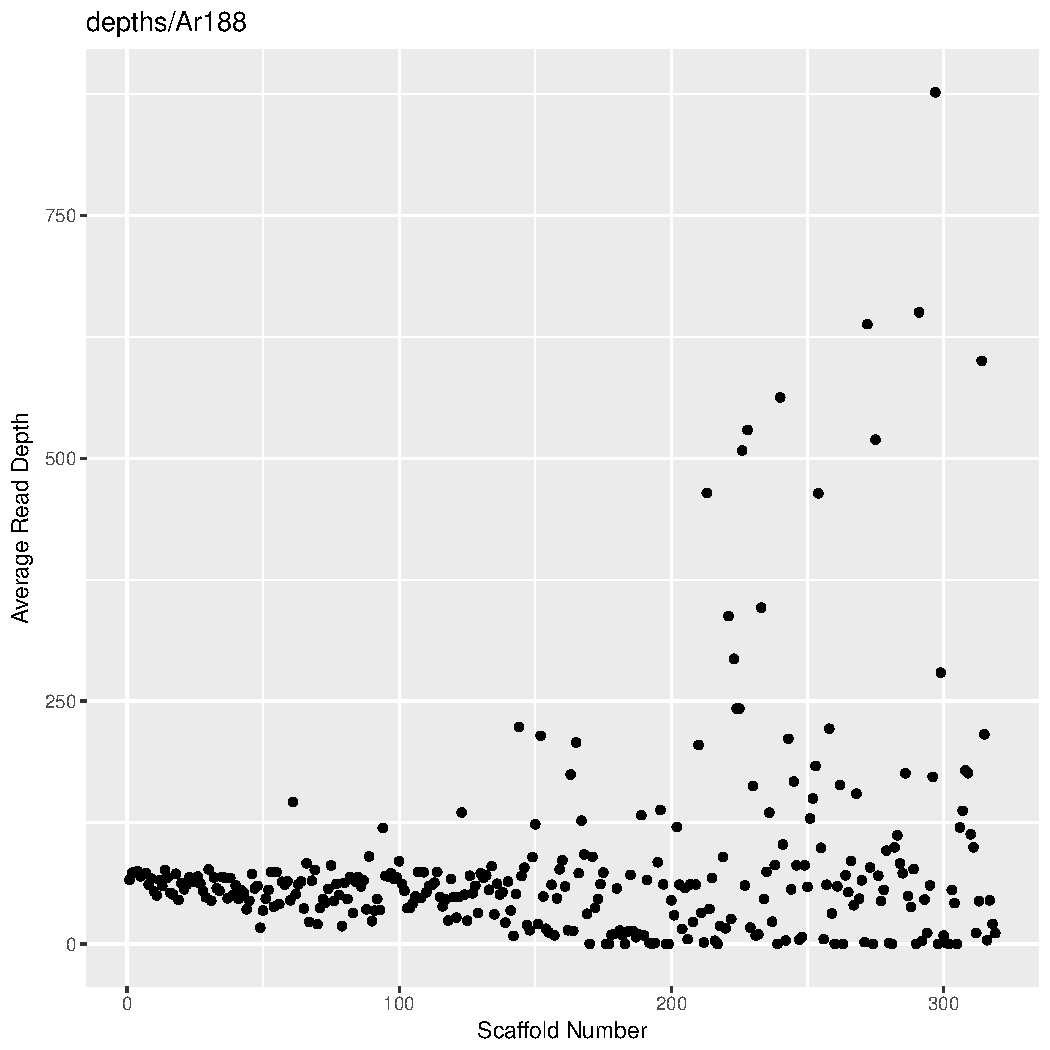
\includegraphics[angle=0,width=1.0\linewidth]{Figures/Ar188_collected_no_comma_read_depth.pdf}}
		\resizebox{78mm}{78mm}{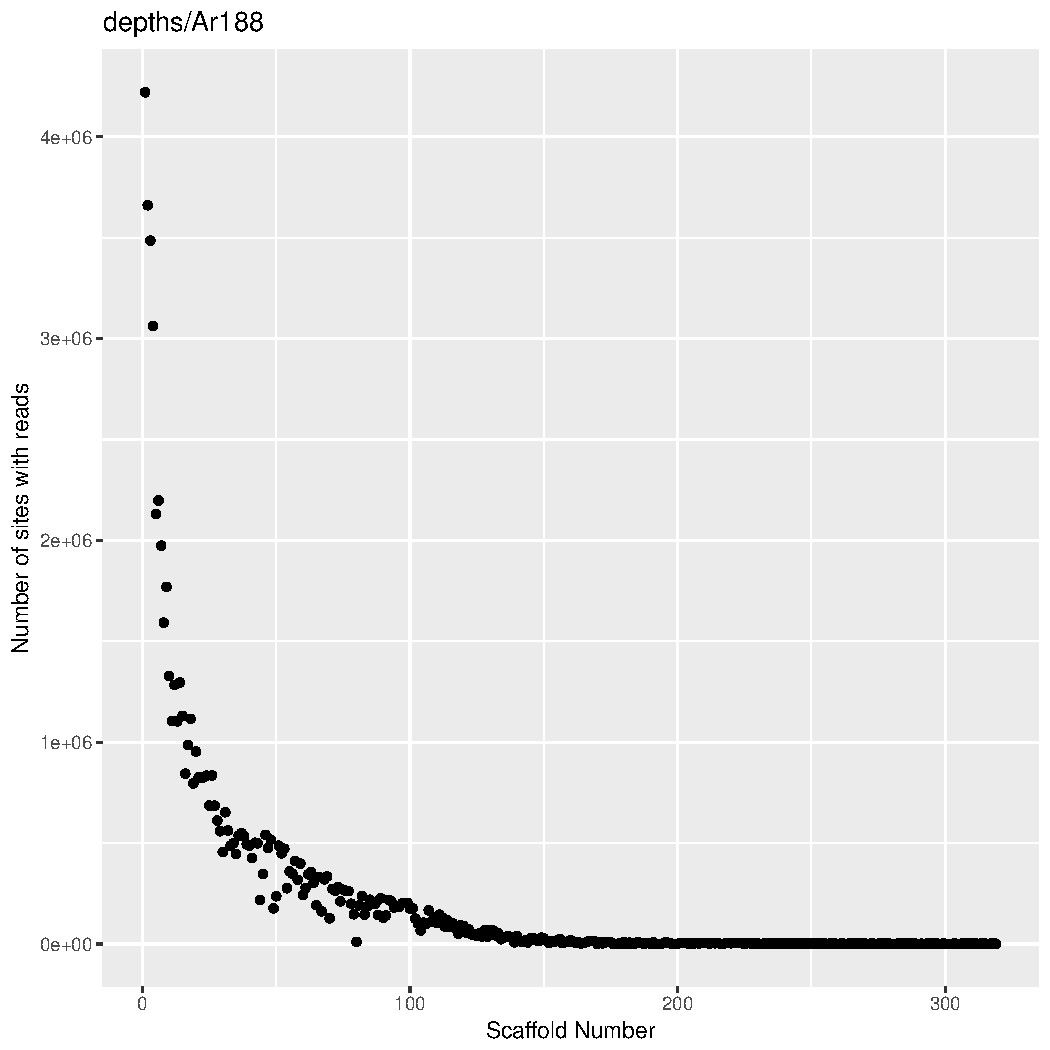
\includegraphics[angle=0,width=1.0\linewidth]{Figures/Ar188_collected_no_comma_count.pdf}}\\
		\resizebox{78mm}{78mm}{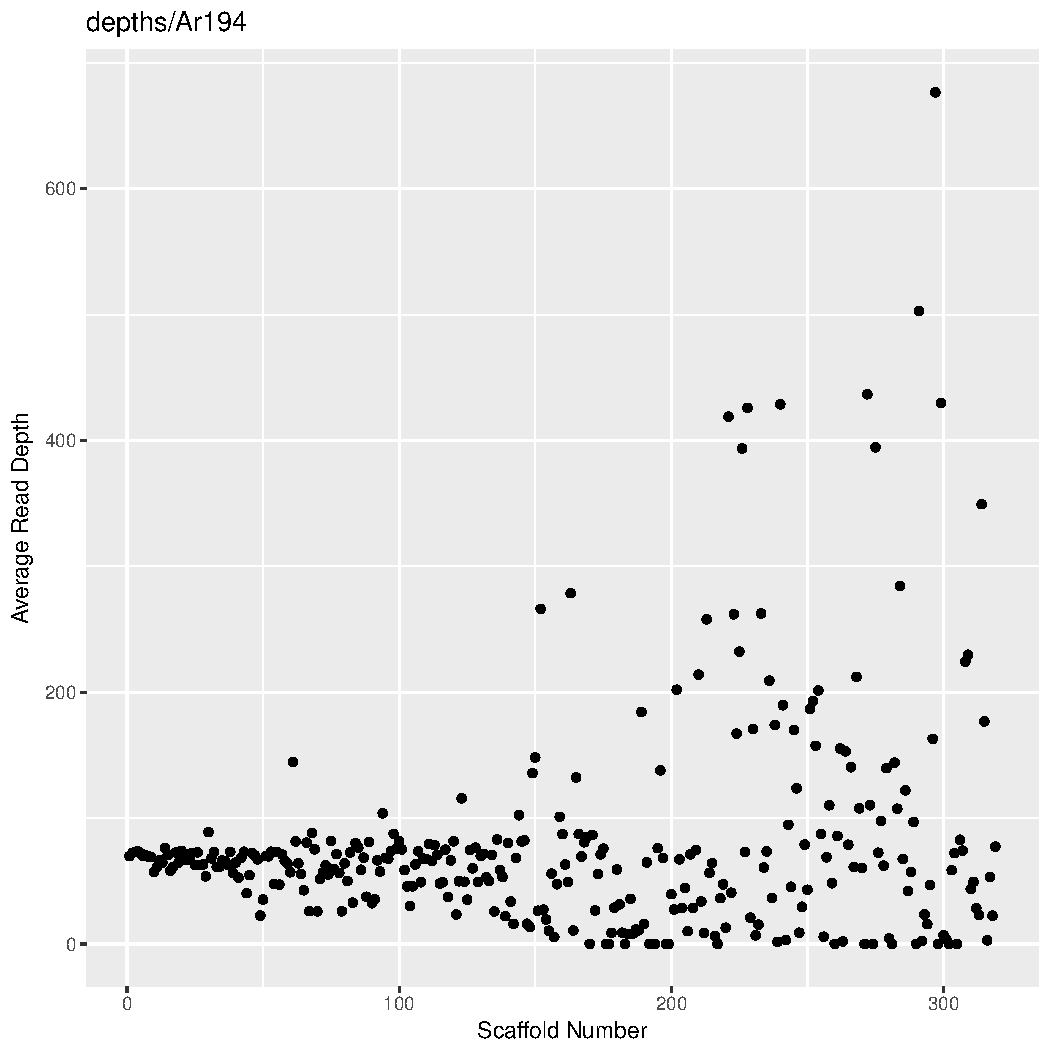
\includegraphics[angle=0,width=1.0\linewidth]{Figures/Ar194_collected_no_comma_read_depth.pdf}}
		\resizebox{78mm}{78mm}{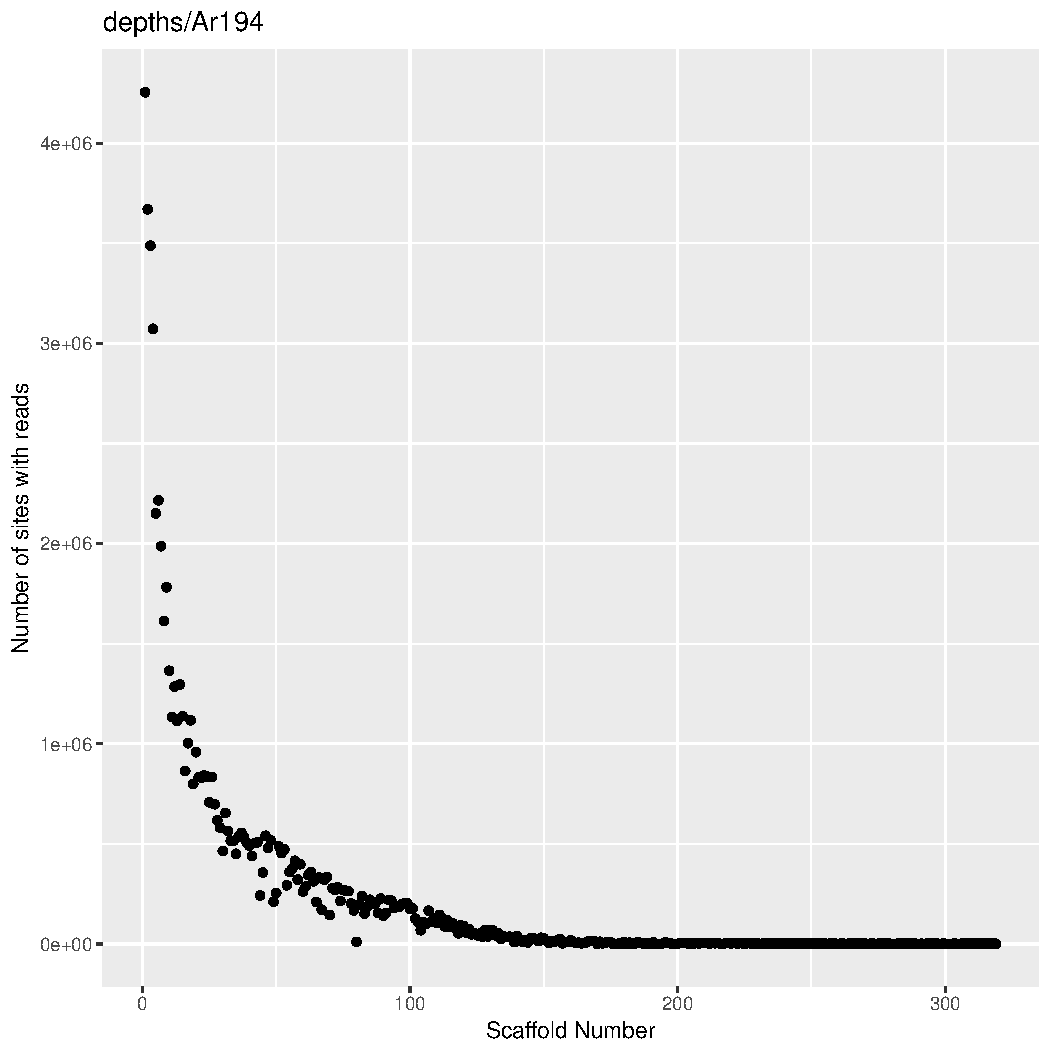
\includegraphics[angle=0,width=1.0\linewidth]{Figures/Ar194_collected_no_comma_count.pdf}}\\
		\begin{singlespace}
			\vspace{-0.5cm}		
			\caption[Average Read Depth Per scaffold, Ar:179, 188, 194]{Average Read Depth Per scaffold, Ar:179, 188, 194. Graphs on the left are the average read depth vs scaffold number and graphs on the right are the total number of sites with reads aligned to them per scaffold.}\label{avg_rd_graphs_4}
		\end{singlespace}	
	\end{centering}
\end{figure}
\begin{figure}[H]
	\begin{centering}
		\vspace{-1.5cm}
		\resizebox{78mm}{78mm}{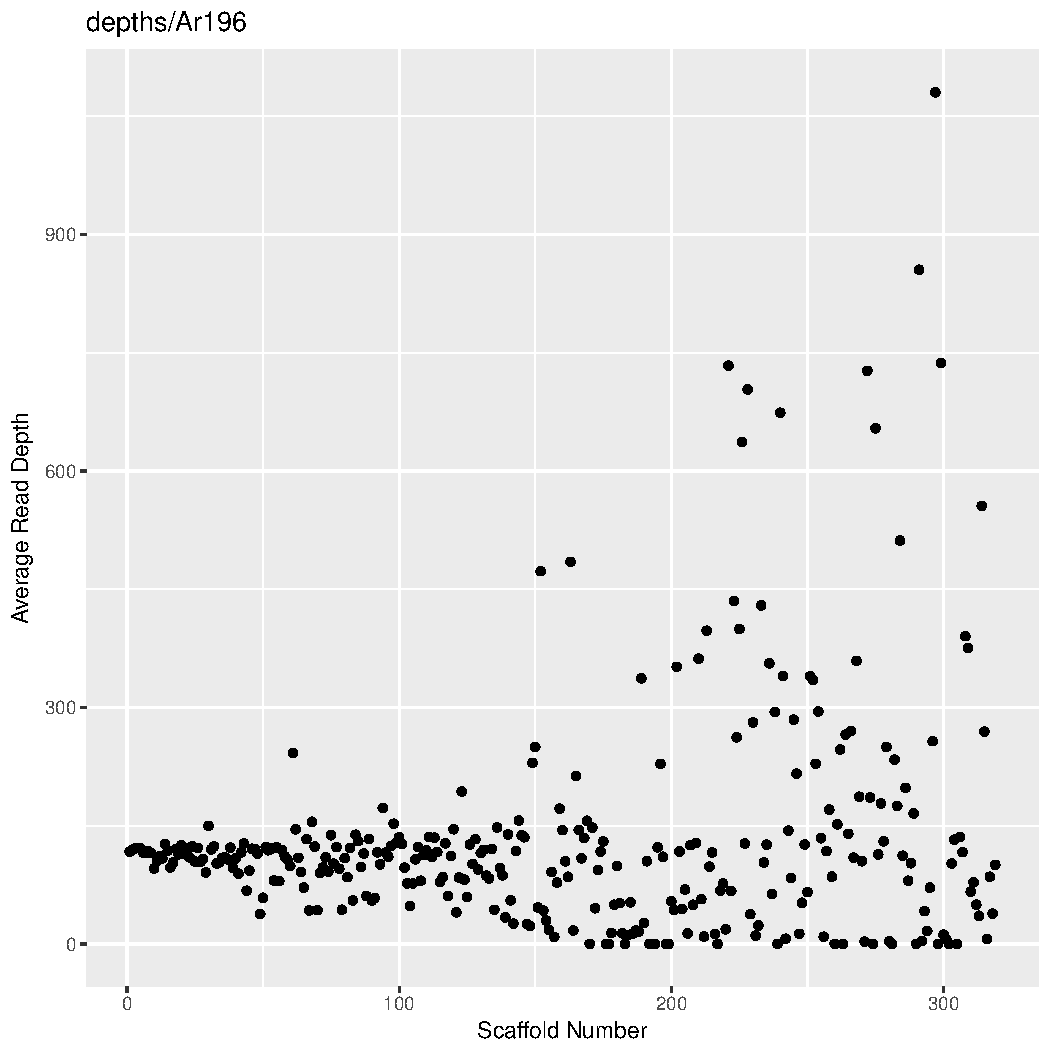
\includegraphics[angle=0,width=1.0\linewidth]{Figures/Ar196_collected_no_comma_read_depth.pdf}}
		\resizebox{78mm}{78mm}{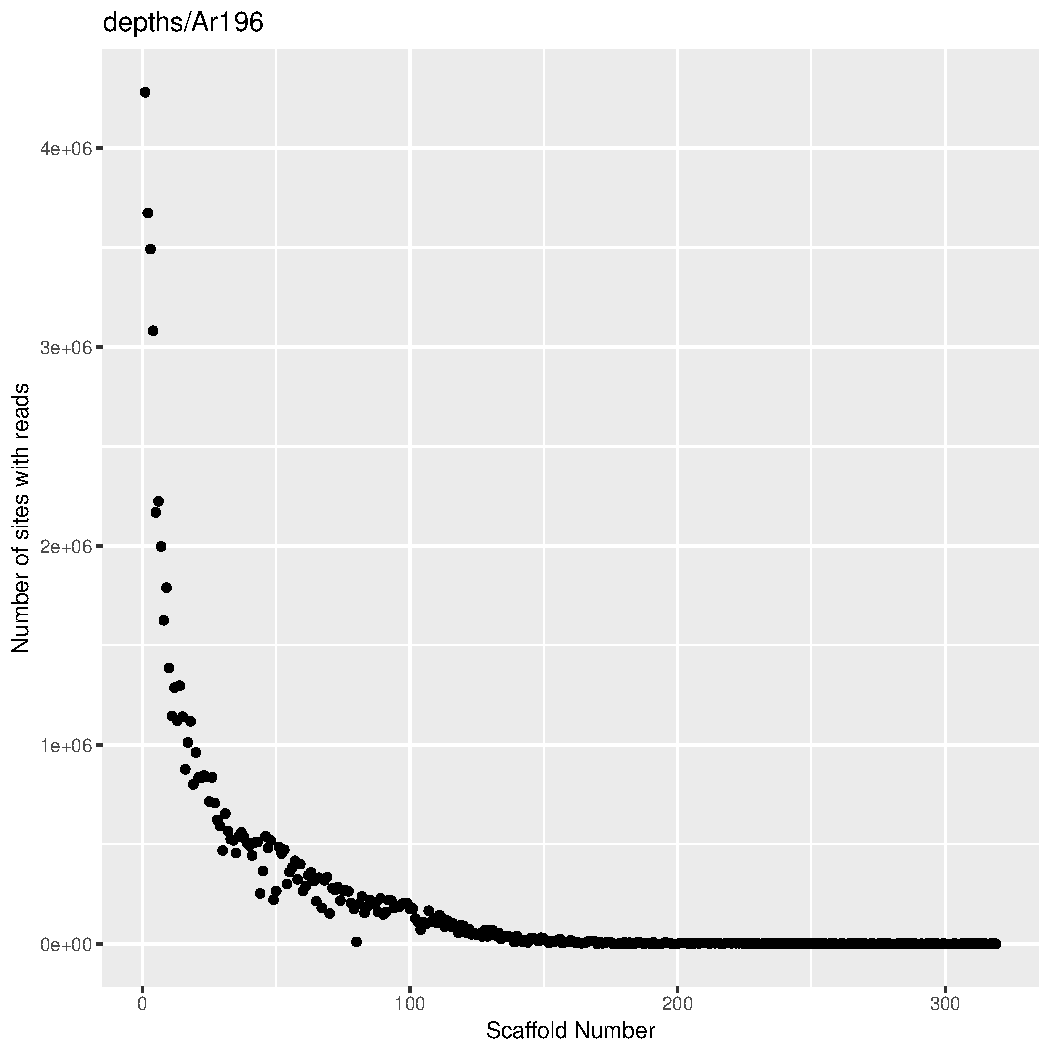
\includegraphics[angle=0,width=1.0\linewidth]{Figures/Ar196_collected_no_comma_count.pdf}}\\
		\resizebox{78mm}{78mm}{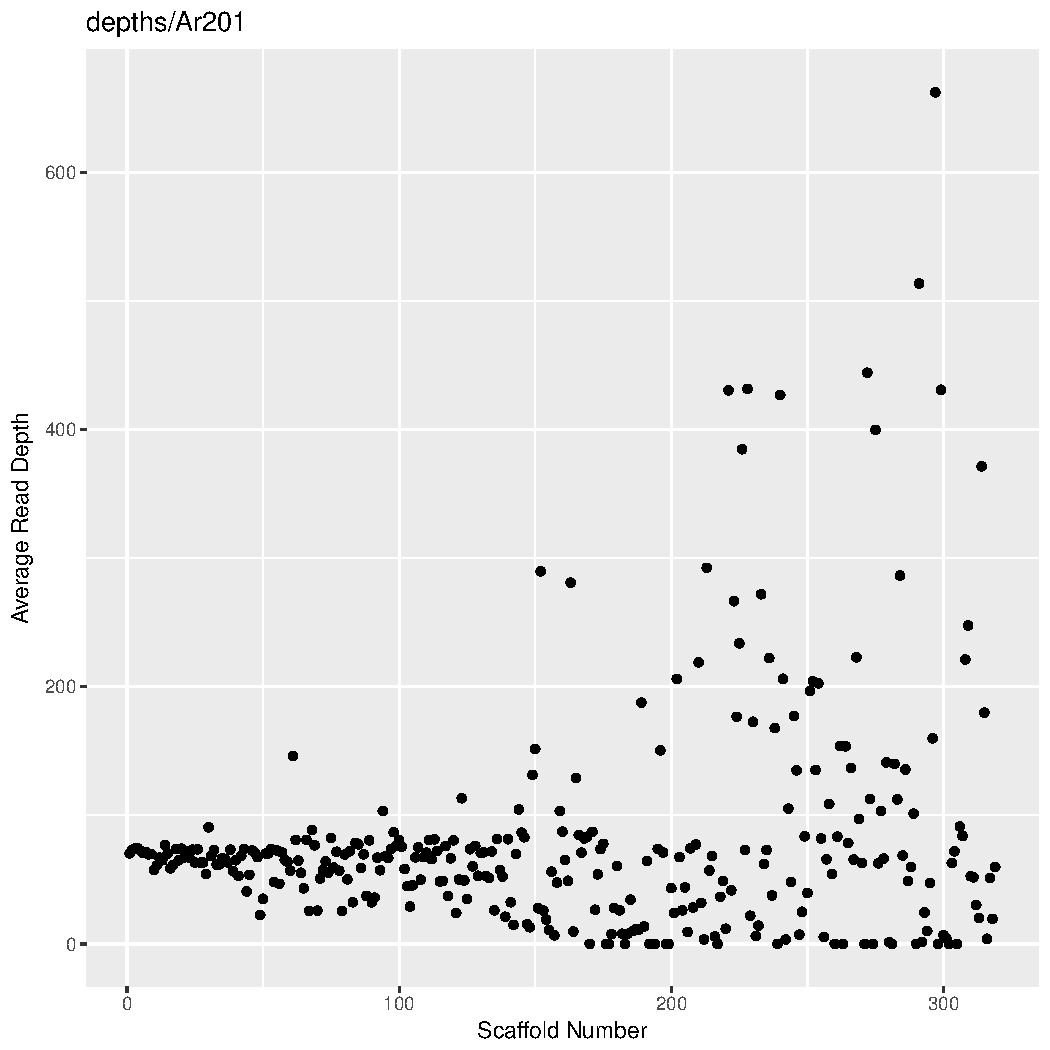
\includegraphics[angle=0,width=1.0\linewidth]{Figures/Ar201_collected_no_comma_read_depth.pdf}}
		\resizebox{78mm}{78mm}{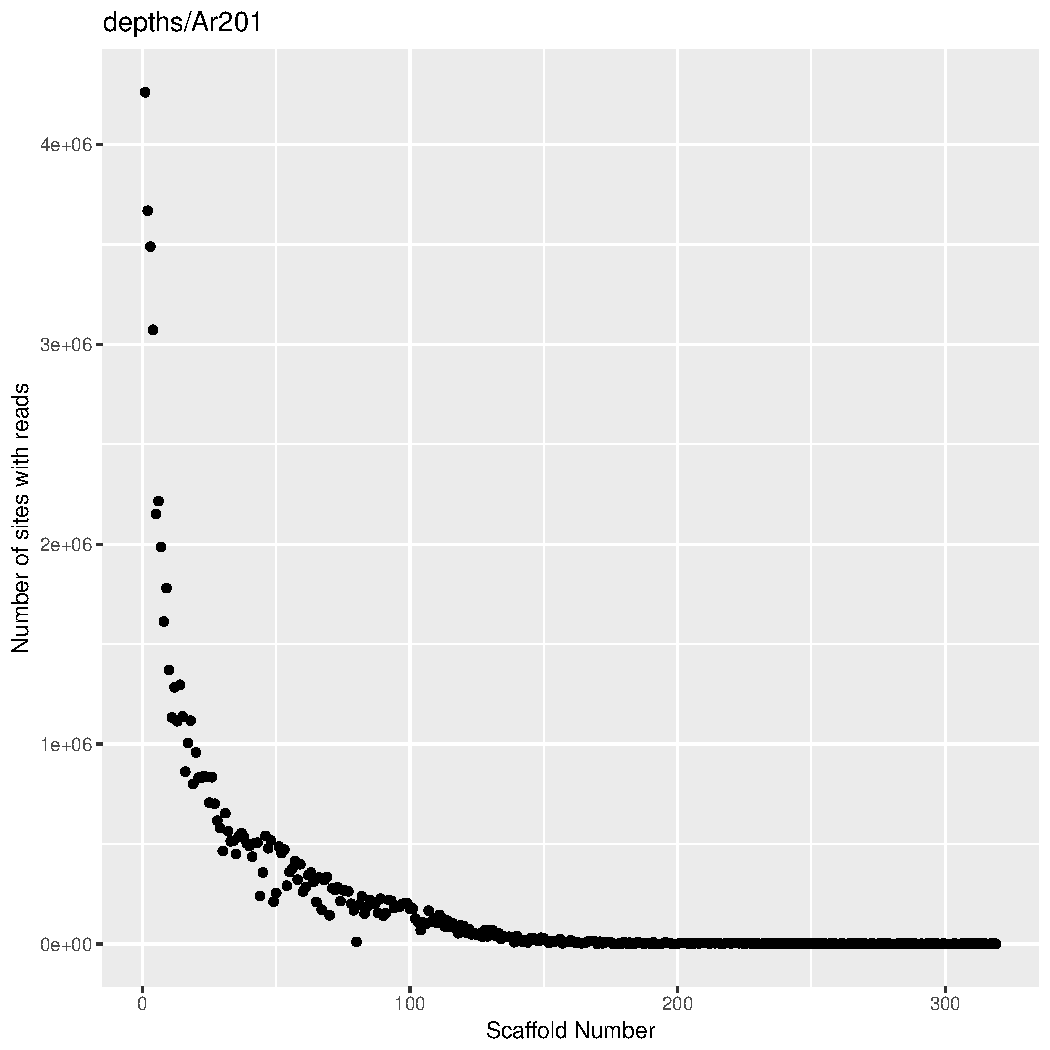
\includegraphics[angle=0,width=1.0\linewidth]{Figures/Ar201_collected_no_comma_count.pdf}}\\
		\resizebox{78mm}{78mm}{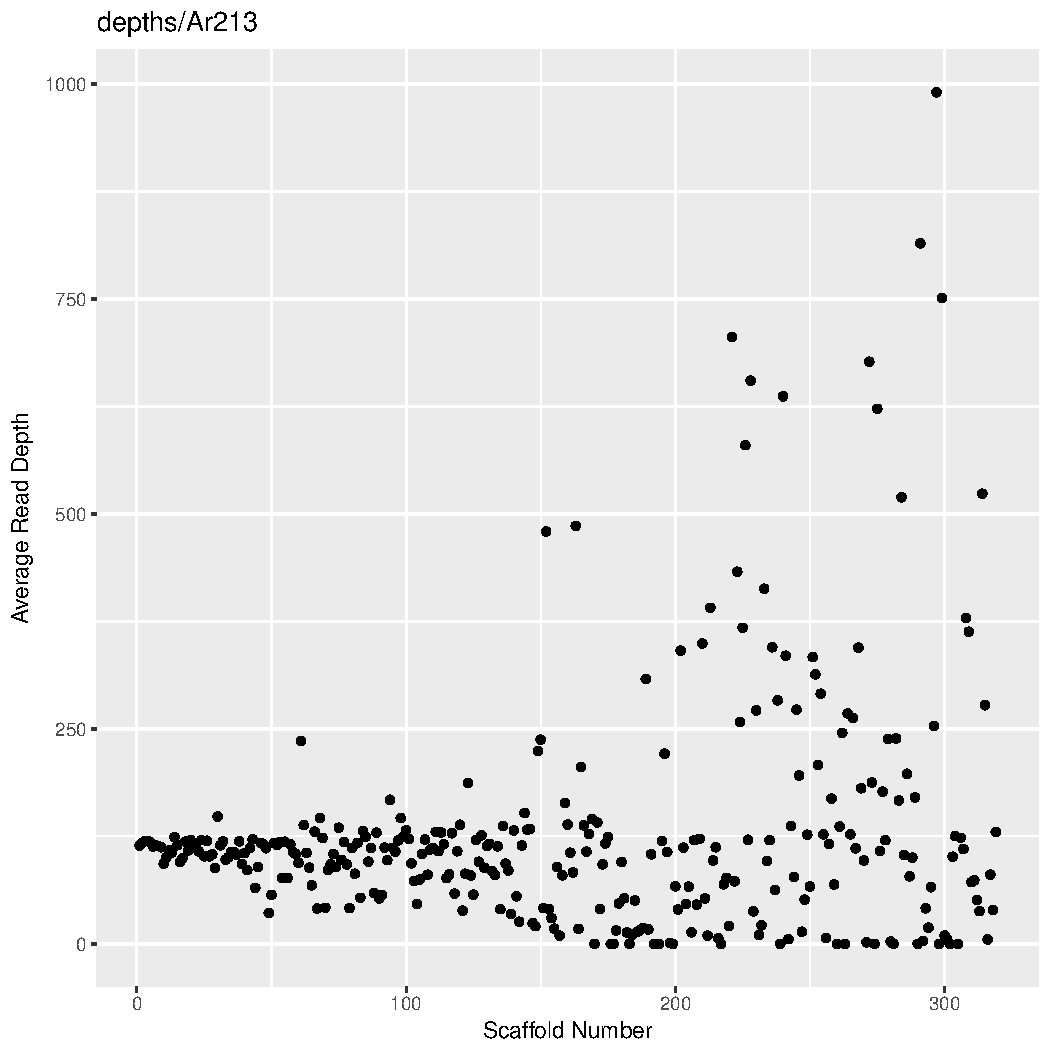
\includegraphics[angle=0,width=1.0\linewidth]{Figures/Ar213_collected_no_comma_read_depth.pdf}}
		\resizebox{78mm}{78mm}{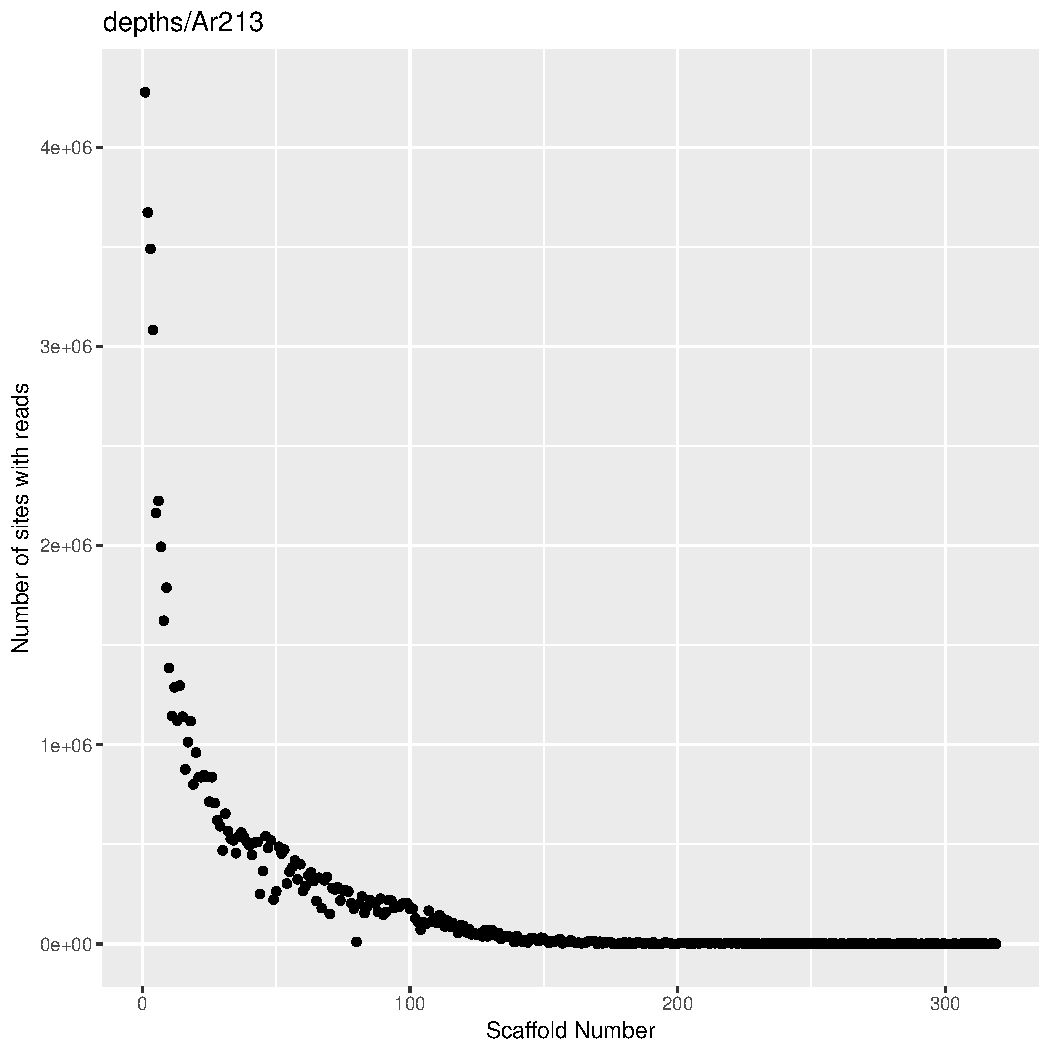
\includegraphics[angle=0,width=1.0\linewidth]{Figures/Ar213_collected_no_comma_count.pdf}}\\
		\begin{singlespace}
			\vspace{-0.5cm}		
			\caption[Average Read Depth Per scaffold, Ar:196, 201, 213]{Average Read Depth Per scaffold, Ar:196, 201, 213. Graphs on the left are the average read depth vs scaffold number and graphs on the right are the total number of sites with reads aligned to them per scaffold.}\label{avg_rd_graphs_5}
		\end{singlespace}	
	\end{centering}
\end{figure}
\newpage

\end{document}
